\documentclass[aspectratio=169,12pt]{beamer}
\usepackage[utf8]{inputenc}
\usepackage[T1]{fontenc}

\usepackage{lmodern}
%\usepackage[]{helvet}
%\usepackage[]{bookman}
%\usepackage[]{newcent}
\usepackage{tikz}
\usepackage{pdfpages}
\usepackage{fancyvrb}
\usepackage{listings}
\usepackage[absolute,overlay]{textpos}

\usetikzlibrary{shapes,arrows,calc,patterns,backgrounds,fit}

\tikzstyle{block} = [draw, text=white!90!gray, fill=blue!20!gray, rectangle, rounded corners, minimum height=2.6em, minimum width=5.5em]
\tikzstyle{sum} = [draw, fill=blue!20, circle, node distance=1cm]
\tikzstyle{input} = [coordinate]
\tikzstyle{output} = [coordinate]
\tikzstyle{pinstyle} = [pin edge={to-,thin,black}]
\tikzstyle{bus} = [thick,double distance=0.1em,>=latex']
\tikzstyle{secnsecreg}=[minimum width=13em,minimum height=2em]
\tikzstyle{secure}=[secnsecreg,fill=blue!50!gray,fill opacity=0.8]
\tikzstyle{nonsecure}=[secnsecreg,fill opacity=0.6,fill=orange]
\tikzstyle{sg}=[secnsecreg,pattern=crosshatch,pattern color=blue!50!gray,fill opacity=0.8]

\colorlet{ltb_green}{green!70!black}
\colorlet{ltb_blue}{blue!75!black}
\colorlet{ltb_orange}{orange!80}
\colorlet{ltb_yellow}{yellow!65!orange}
\colorlet{ltb_red}{red!80!black}
\colorlet{ltb_highlight_red}{ltb_red}
\colorlet{ltb_highlight_orange}{ltb_orange}
\tikzstyle{ltb_blue_trans}=[fill=blue!25,fill opacity=0.5]
\tikzstyle{ltb_orange_trans}=[fill opacity=0.5,fill=orange]

\makeatletter
\@ifclassloaded{beamer}{
    \newcommand{\ltbbeamer}[0]{1=1}
}{
    \newcommand{\ltbbeamer}[0]{1=0}
}
\makeatother
\newcommand{\mytikzrefnode}[1]{\tikz[remember picture,baseline=-.5ex] \coordinate (#1) {};}

\tikzstyle{every picture}+=[remember picture]
\tikzset{font={\fontsize{10pt}{12}\selectfont}}
\newcommand{\ltbtextblue}[1]{\textcolor{ltb_blue}{#1}}
\newcommand{\ltbtextbluebf}[1]{\textcolor{ltb_blue}{\bf{}#1}}
\newcommand{\ltbtextbluett}[1]{\textcolor{ltb_blue}{\tt{}#1}}
\newcommand{\ltbtextorange}[1]{\textcolor{ltb_orange}{#1}}
\newcommand{\ltbtextorangebf}[1]{\textcolor{ltb_orange}{\bf{}#1}}
\newcommand{\ltbtextorangett}[1]{\textcolor{ltb_orange}{\tt{}#1}}
\newcommand{\ltbtextgreentt}[1]{\textcolor{ltb_green}{\tt{}#1}}

%\usetheme{Berlin}
%\usetheme{Warsaw}
\usetheme{Frankfurt}

\title{JTAG Switcher}
\author{Alexander Merkle - Lauterbach GmbH}
\newcommand{\gitdate}{__GITDATE__}

\date{\gitdate}

\begin{document}

\begin{frame}
\titlepage
\end{frame}

\begin{frame}
\frametitle{Overview}
\tableofcontents[hideallsubsections]
\end{frame}

%==============================

\begin{frame}[t]{Abbreviations}
\begin{itemize}
\item TAP: Test-Access-Port, JTAG communication unit, consists of Instruction- \& multiple Data-Registers selected by a state-machine
\item Daisy-Chain: connection of multiple TAPs via a single interface
\item JTAG Signals:
\begin{itemize}
\item \texttt{TCK: }Test Clock, clocks all D-flip-flops, which are part of the JTAG architecture
\item \texttt{TMS: }Test Machine State, controls the JTAG TAP Controller state machine
\item \texttt{TDI: }Test Data In, serial data send into the JTAG architecture
\item \texttt{TDO: }Test Data Out, serial data received from the JTAG architecture
\item \texttt{TRST*:} Test Reset, optional, will \emph{asynchronously} reset the JTAG TAP Controller state machine,
putting it into the "Test-Logic-Reset" state
\end{itemize}
\end{itemize}
\end{frame}

\section{JTAG Daisy-Chaining Basics}

\begin{frame}[t]{Simple Daisy-Chain}
\begin{center}
\newcommand{\jtag}[2]
{
\node [jnode,anchor=west] (jtag#1) at #2 {};
\node [right] at ([yshift=0.5em]jtag#1.west) (_jtag#1_tdi) {TDI};
\node [left] at ([yshift=0.5em]jtag#1.east) (_jtag#1_tdo) {TDO};
\node [above] at ([xshift=-1.5em]jtag#1.south) (_jtag#1_tck)  {TCK};
\node [above] at ([xshift=1.5em]jtag#1.south) (_jtag#1_tms) {TMS};
\coordinate (jtag#1_tdi) at (_jtag#1_tdi.west);
\coordinate (jtag#1_tdo) at (_jtag#1_tdo.east);
\coordinate (jtag#1_tck) at (_jtag#1_tck.south);
\coordinate (jtag#1_tms) at (_jtag#1_tms.south);
}
\tikzstyle{jnode}=[draw,rounded corners,minimum height=3.5em,minimum width=8em]
\tikzstyle{buffer}=[draw=black,fill=white,regular polygon,regular polygon sides=3,rotate=30,inner sep=0,minimum height=1.5em]

\tikzstyle{demux} = [trapezium,draw,shape border rotate=90,trapezium stretches body]
\tikzstyle{mux} = [trapezium,draw,shape border rotate=270,trapezium stretches body]

\begin{tikzpicture}[]
\jtag{1}{(0,0)}
\jtag{2}{([xshift=3em]jtag1.east)}
\jtag{3}{([xshift=3em]jtag2.east)}

\path (jtag1_tck) to ++(0,-1.5em) coordinate (tck_inters) -- ++(0,-3.5em) coordinate (tck_in);
\path (jtag1_tms) to ++(0,-2.5em) coordinate (tms_inters) -- (tck_in -| jtag1_tms) coordinate (tms_in);
\coordinate (tdi_in) at ($(tms_in)!2!(tck_in)$);
\coordinate (tdo_in) at ($(tck_in)!2!(tms_in)$);

\node [below] at (tdi_in) {TDI};
\node [below] at (tck_in) {TCK};
\node [below] at (tms_in) {TMS};
\node [below] at (tdo_in) {TDO};

\draw [->,thick] (jtag1_tdo) -- (jtag2_tdi);
\draw [->,thick] (jtag2_tdo) -- (jtag3_tdi);

\draw [<-,thick] (jtag1_tdi) -| ([xshift=-1.5em]jtag1.south west) -- +(0,-3.5em) -| (tdi_in);
\draw [->,thick] (jtag3_tdo) -|  ([xshift=1.5em]jtag3.south east) -- +(0,-3.5em) -| (tdo_in);
\draw [->,thick] (tck_in) -- (jtag1_tck);
\draw [->,thick] (tms_in) -- (jtag1_tms);
\draw [fill] (tms_inters) circle (0.15em);
\draw [fill] (tck_inters) circle (0.15em);
\draw [->,thick] (tck_inters) -| (jtag2_tck);
\draw [->,thick] (tck_inters) -| (jtag3_tck);
\draw [->,thick] (tms_inters) -| (jtag2_tms);
\draw [->,thick] (tms_inters) -| (jtag3_tms);

\end{tikzpicture}
\end{center}
\begin{itemize}
\item A Daisy-Chain is formed by connecting TDO to TDI of the next TAP controller
\item TCK \& TMS are shared signals
\end{itemize}
\end{frame}

\begin{frame}[t]{Simple Daisy-Chain}
\begin{center}
\newcommand{\jtag}[2]
{
\node [jnode,anchor=west] (jtag#1) at #2 {};
\node [right] at ([yshift=0.5em]jtag#1.west) (_jtag#1_tdi) {TDI};
\node [left] at ([yshift=0.5em]jtag#1.east) (_jtag#1_tdo) {TDO};
\node [above] at ([xshift=-1.5em]jtag#1.south) (_jtag#1_tck)  {TCK};
\node [above] at ([xshift=1.5em]jtag#1.south) (_jtag#1_tms) {TMS};
\coordinate (jtag#1_tdi) at (_jtag#1_tdi.west);
\coordinate (jtag#1_tdo) at (_jtag#1_tdo.east);
\coordinate (jtag#1_tck) at (_jtag#1_tck.south);
\coordinate (jtag#1_tms) at (_jtag#1_tms.south);
}
\tikzstyle{jnode}=[draw,rounded corners,minimum height=3.5em,minimum width=8em]
\tikzstyle{buffer}=[draw=black,fill=white,regular polygon,regular polygon sides=3,rotate=30,inner sep=0,minimum height=1.5em]

\tikzstyle{demux} = [trapezium,draw,shape border rotate=90,trapezium stretches body]
\tikzstyle{mux} = [trapezium,draw,shape border rotate=270,trapezium stretches body]

\begin{tikzpicture}[]
\jtag{1}{(0,0)}
\jtag{2}{([xshift=3em]jtag1.east)}
\jtag{3}{([xshift=3em]jtag2.east)}

\path (jtag1_tck) to ++(0,-1.5em) coordinate (tck_inters) -- ++(0,-3.5em) coordinate (tck_in);
\path (jtag1_tms) to ++(0,-2.5em) coordinate (tms_inters) -- (tck_in -| jtag1_tms) coordinate (tms_in);
\coordinate (tdi_in) at ($(tms_in)!2!(tck_in)$);
\coordinate (tdo_in) at ($(tck_in)!2!(tms_in)$);

\node [below] at (tdi_in) {TDI};
\node [below] at (tck_in) {TCK};
\node [below] at (tms_in) {TMS};
\node [below] at (tdo_in) {TDO};

\draw [->,thick] (jtag1_tdo) -- (jtag2_tdi);
\draw [->,thick] (jtag2_tdo) -- (jtag3_tdi);

\draw [<-,thick] (jtag1_tdi) -| ([xshift=-1.5em]jtag1.south west) -- +(0,-2.5em) -| (tdi_in);
\draw [->,thick] (jtag3_tdo) -|  ([xshift=1.5em]jtag3.south east) -- +(0,-2.5em) -| (tdo_in);
%\draw [->,thick] (tck_in) -- (jtag1_tck);
\draw [->,thick] (tck_in) -- ++(0,.6em) node [draw,minimum height=2em,minimum width=2em,anchor=south,fill=white] (tck_buf) {};
\draw [<-,thick] ($(tck_buf.south west)!0.25!(tck_buf.south east)$) -- +(0,-0.35em) -| (tck_in);
\draw [<-,thick] ($(tck_buf.south west)!0.75!(tck_buf.south east)$) -- +(0,-0.35em) -| (tck_in);
\coordinate (tck_buf_out1) at ($(tck_buf.north west)!0.25!(tck_buf.north east)$);
\coordinate (tck_buf_out2) at ($(tck_buf.north west)!0.5!(tck_buf.north east)$);
\coordinate (tck_buf_out3) at ($(tck_buf.north west)!0.75!(tck_buf.north east)$);
\node [buffer] at (tck_buf) {};

\draw [->,thick] (tms_in) -- ++(0,.6em) node [draw,minimum height=2em,minimum width=2em,anchor=south,fill=white] (tms_buf) {};
\draw [<-,thick] ($(tms_buf.south west)!0.25!(tms_buf.south east)$) -- +(0,-0.35em) -| (tms_in);
\draw [<-,thick] ($(tms_buf.south west)!0.75!(tms_buf.south east)$) -- +(0,-0.35em) -| (tms_in);
\coordinate (tms_buf_out1) at ($(tms_buf.north west)!0.25!(tms_buf.north east)$);
\coordinate (tms_buf_out2) at ($(tms_buf.north west)!0.5!(tms_buf.north east)$);
\coordinate (tms_buf_out3) at ($(tms_buf.north west)!0.75!(tms_buf.north east)$);
\node [buffer] at (tms_buf) {};

\draw [thick,->] (tck_buf_out1) edge [->] ++(0,0.35em) |- (tck_buf_out1 |- jtag1_tck);
\draw [thick,->] (tck_buf_out2) edge [->] ++(0,0.35em) ++(0,0.35em) |- ([yshift=-0.6em]jtag2_tck) -- (jtag2_tck);
\draw [thick,->] (tck_buf_out3) edge [->] ++(0,0.35em) ++(0,0.35em) |- ([yshift=-0.8em]jtag3_tck) -- (jtag3_tck);
\draw [thick,->] (tms_buf_out1) edge [->] ++(0,0.35em) |- (tms_buf_out1 |- jtag1_tms);
\draw [thick,->] (tms_buf_out2) edge [->] ++(0,0.35em) ++(0,0.35em) |- ([yshift=-1.2em]jtag2_tms) -- (jtag2_tms);
\draw [thick,->] (tms_buf_out3) edge [->] ++(0,0.35em) ++(0,0.35em) |- ([yshift=-1.4em]jtag3_tms) -- (jtag3_tms);

\end{tikzpicture}
\end{center}
\begin{block}{Recommendation}
Do not route TCK/TMS as a STAR (stub wires cause reflections).\\
Use a buffer with one output per TAP for signal integrity.
\end{block}
\begin{tikzpicture}[overlay]
\node [draw,rounded corners,thick,inner sep=0.5em,ltb_blue,fit=(tck_buf)(tms_buf)] {};
\end{tikzpicture}
\end{frame}

\begin{frame}[t]{Real world Daisy-Chain}
\vspace{-2.5em}
\begin{center}
\newcommand{\jtag}[2]
{
\node [jnode,anchor=west] (jtag#1) at #2 {};
\node [right] at ([yshift=0.5em]jtag#1.west) (_jtag#1_tdi) {TDI};
\node [left] at ([yshift=0.5em]jtag#1.east) (_jtag#1_tdo) {TDO};
\node [above] at ([xshift=-1.5em]jtag#1.south) (_jtag#1_tck)  {TCK};
\node [above] at ([xshift=1.5em]jtag#1.south) (_jtag#1_tms) {TMS};
\coordinate (jtag#1_tdi) at (_jtag#1_tdi.west);
\coordinate (jtag#1_tdo) at (_jtag#1_tdo.east);
\coordinate (jtag#1_tck) at (_jtag#1_tck.south);
\coordinate (jtag#1_tms) at (_jtag#1_tms.south);
}
\tikzstyle{jnode}=[draw,rounded corners,minimum height=3.5em,minimum width=8em]
\tikzstyle{buffer}=[draw=black,fill=white,regular polygon,regular polygon sides=3,rotate=30,inner sep=0,minimum height=1.5em]

\tikzstyle{demux} = [trapezium,draw,shape border rotate=90,trapezium stretches body]
\tikzstyle{mux} = [trapezium,draw,shape border rotate=270,trapezium stretches body]

\begin{tikzpicture}[inner frame sep=0]
%\begin{tikzpicture}[show background rectangle,inner frame sep=0]
\jtag{1}{(0,0)}
\jtag{2}{([xshift=3em]jtag1.east)}
\jtag{3}{([xshift=3em]jtag2.east)}

\path (jtag1_tck) to ++(0,-1.5em) coordinate (tck_inters) -- ++(0,-3.5em) coordinate (tck_in);
\path (jtag1_tms) to ++(0,-2.5em) coordinate (tms_inters) -- (tck_in -| jtag1_tms) coordinate (tms_in);
\coordinate (tdi_in) at ($(tms_in)!2!(tck_in)$);
\coordinate (tdo_in) at ($(tck_in)!2!(tms_in)$);

\node [below] at (tdi_in) {TDI};
\node [below] at (tck_in) {TCK};
\node [below] at (tms_in) {TMS};
\node [below] at (tdo_in) {TDO};

\draw [->,thick] (jtag1_tdo) -- node [buffer] {} (jtag2_tdi);
\draw [->,thick] (jtag2_tdo) -- node [buffer] {} (jtag3_tdi);

\draw [<-,thick] (jtag1_tdi) -| ([xshift=-1.5em]jtag1.south west) -- +(0,-2.5em) -| (tdi_in);
\draw [->,thick] (jtag3_tdo) -|  ([xshift=1.5em]jtag3.south east) -- +(0,-2.5em) -| (tdo_in);
%\draw [->,thick] (tck_in) -- (jtag1_tck);
\draw [->,thick] (tck_in) -- ++(0,.6em) node [draw,minimum height=2em,minimum width=2em,anchor=south,fill=white] (tck_buf) {};
\draw [<-,thick] ($(tck_buf.south west)!0.25!(tck_buf.south east)$) -- +(0,-0.35em) -| (tck_in);
\draw [<-,thick] ($(tck_buf.south west)!0.75!(tck_buf.south east)$) -- +(0,-0.35em) -| (tck_in);
\coordinate (tck_buf_out1) at ($(tck_buf.north west)!0.25!(tck_buf.north east)$);
\coordinate (tck_buf_out2) at ($(tck_buf.north west)!0.5!(tck_buf.north east)$);
\coordinate (tck_buf_out3) at ($(tck_buf.north west)!0.75!(tck_buf.north east)$);
\node [buffer] at (tck_buf) {};

\draw [->,thick] (tms_in) -- ++(0,.6em) node [draw,minimum height=2em,minimum width=2em,anchor=south,fill=white] (tms_buf) {};
\draw [<-,thick] ($(tms_buf.south west)!0.25!(tms_buf.south east)$) -- +(0,-0.35em) -| (tms_in);
\draw [<-,thick] ($(tms_buf.south west)!0.75!(tms_buf.south east)$) -- +(0,-0.35em) -| (tms_in);
\coordinate (tms_buf_out1) at ($(tms_buf.north west)!0.25!(tms_buf.north east)$);
\coordinate (tms_buf_out2) at ($(tms_buf.north west)!0.5!(tms_buf.north east)$);
\coordinate (tms_buf_out3) at ($(tms_buf.north west)!0.75!(tms_buf.north east)$);
\node [buffer] at (tms_buf) {};

\draw [thick,->] (tck_buf_out1) edge [->] ++(0,0.35em) |- (tck_buf_out1 |- jtag1_tck);
\draw [thick,->] (tck_buf_out2) edge [->] ++(0,0.35em) ++(0,0.35em) |- ([yshift=-0.6em]jtag2_tck) -- (jtag2_tck);
\draw [thick,->] (tck_buf_out3) edge [->] ++(0,0.35em) ++(0,0.35em) |- ([yshift=-0.8em]jtag3_tck) -- (jtag3_tck);
\draw [thick,->] (tms_buf_out1) edge [->] ++(0,0.35em) |- (tms_buf_out1 |- jtag1_tms);
\draw [thick,->] (tms_buf_out2) edge [->] ++(0,0.35em) ++(0,0.35em) |- ([yshift=-1.2em]jtag2_tms) -- (jtag2_tms);
\draw [thick,->] (tms_buf_out3) edge [->] ++(0,0.35em) ++(0,0.35em) |- ([yshift=-1.4em]jtag3_tms) -- (jtag3_tms);

\path (tdi_in) |- node [thick,buffer,rotate=-30,yshift=-0.1em] (tdi_in_buf) {} (tck_buf.west);
\path (tdo_in) |- node [thick,buffer,rotate=30] (tdo_in_buf) {} (tck_buf.west);

\ifthenelse{\ltbbeamer}{
	\node [draw=ltb_red,rounded corners,fit=(jtag1),label={\tiny{}VREF=?V}] {};
	\node [draw=ltb_blue,rounded corners,fit=(jtag2),label={\tiny{}VREF=?V}] {};
	\node [draw=ltb_green,rounded corners,fit=(jtag3),label={\tiny{}VREF=?V}] {};
}{
	\node [fit=(jtag1),label={\tiny{}IC 1 - $VREF_1$}] {};
	\node [fit=(jtag2),label={\tiny{}IC 2 - $VREF_2$}] {};
	\node [fit=(jtag3),label={\tiny{}IC 3 - $VREF_3$}] {};
}
\begin{scope}[on background layer]
	\draw [dashed,gray] ([xshift=-4em]tck_buf.west) -- (tck_buf.west -| tdo_in_buf) -- +(2em,0) node [below,xshift=1em] {\tiny{}VREF=?V};
\end{scope}
\end{tikzpicture}
\end{center}
\begin{itemize}
\item In case of different I/O Voltages multiple level shifters are required
\end{itemize}
\end{frame}

\begin{frame}[t]{FPGA Implementation}
\begin{center}
\newcommand{\jtag}[2]
{
\node [jnode,anchor=west] (jtag#1) at #2 {};
\node [right] at ([yshift=0.5em]jtag#1.west) (_jtag#1_tdi) {TDI};
\node [left] at ([yshift=0.5em]jtag#1.east) (_jtag#1_tdo) {TDO};
\node [above] at ([xshift=-1.5em]jtag#1.south) (_jtag#1_tck)  {TCK};
\node [above] at ([xshift=1.5em]jtag#1.south) (_jtag#1_tms) {TMS};
\coordinate (jtag#1_tdi) at (_jtag#1_tdi.west);
\coordinate (jtag#1_tdo) at (_jtag#1_tdo.east);
\coordinate (jtag#1_tck) at (_jtag#1_tck.south);
\coordinate (jtag#1_tms) at (_jtag#1_tms.south);
}
\tikzstyle{jnode}=[draw,rounded corners,minimum height=3.5em,minimum width=8em]
\tikzstyle{buffer}=[draw=black,fill=white,regular polygon,regular polygon sides=3,rotate=30,inner sep=0,minimum height=1.5em]

\tikzstyle{demux} = [trapezium,draw,shape border rotate=90,trapezium stretches body]
\tikzstyle{mux} = [trapezium,draw,shape border rotate=270,trapezium stretches body]

\begin{tikzpicture}[]
\jtag{1}{(0,0)}
\jtag{2}{([xshift=3em]jtag1.east)}
\jtag{3}{([xshift=3em]jtag2.east)}

\draw ($(jtag1.south west)+(-1.5em,-1.5em)$) coordinate (fpga_north_west) -- ($(jtag3.south east)+(1.5em,-1.5em)$) coordinate (fpga_north_east);
\draw (fpga_north_west) -- +(0,-3em);
\draw (fpga_north_east) -- +(0,-3em) node [anchor=south east] {FPGA};

\draw [thick] (jtag1_tdo) -| ([xshift=0.5em]jtag1_tdo |- fpga_north_west) coordinate (iobank1_tdo);
\draw [thick] (jtag1_tdi) -| ([xshift=-0.5em]jtag1_tdi |- fpga_north_west) coordinate (iobank1_tdi);
\draw [thick] (jtag1_tms) -- (jtag1_tms |- fpga_north_west);
\draw [thick] (jtag1_tck) -- (jtag1_tck |- fpga_north_west);
\draw ([xshift=-0.5em]iobank1_tdi) -- ++(0,-1.5em) coordinate (iobank1_vccio) -| node [yshift=0.3em,anchor=base east] {\tiny{IO-Bank}} ([xshift=0.5em]iobank1_tdo);

\draw [thick] (jtag2_tdo) -| ([xshift=0.5em]jtag2_tdo |- fpga_north_west) coordinate (iobank2_tdo);
\draw [thick] (jtag2_tdi) -| ([xshift=-0.5em]jtag2_tdi |- fpga_north_west) coordinate (iobank2_tdi);
\draw [thick] (jtag2_tms) -- (jtag2_tms |- fpga_north_west);
\draw [thick] (jtag2_tck) -- (jtag2_tck |- fpga_north_west);
\draw ([xshift=-0.5em]iobank2_tdi) -- ++(0,-1.5em) coordinate (iobank2_vccio) -| node [yshift=0.3em,anchor=base east] {\tiny{IO-Bank}} ([xshift=0.5em]iobank2_tdo);

\draw [thick] (jtag3_tdo) -| ([xshift=0.5em]jtag3_tdo |- fpga_north_west) coordinate (iobank3_tdo);
\draw [thick] (jtag3_tdi) -| ([xshift=-0.5em]jtag3_tdi |- fpga_north_west) coordinate (iobank3_tdi);
\draw [thick] (jtag3_tms) -- (jtag3_tms |- fpga_north_west);
\draw [thick] (jtag3_tck) -- (jtag3_tck |- fpga_north_west);
\draw ([xshift=-0.5em]iobank3_tdi) -- ++(0,-1.5em) coordinate (iobank3_vccio) -| node [yshift=0.3em,anchor=base east] {\tiny{IO-Bank}} ([xshift=0.5em]iobank3_tdo);

\node [draw=ltb_red,rounded corners,fit=(jtag1),label={\tiny{}$VREF_1$}] {};
\node [draw=ltb_blue,rounded corners,fit=(jtag2),label={\tiny{}$VREF_2$}] {};
\node [draw=ltb_green,rounded corners,fit=(jtag3),label={\tiny{}$VREF_3$}] {};
\node [yshift=0.3em,anchor=base west] at (iobank1_vccio) {\tiny{}$VCC_{IO}=VREF_1$};
\node [yshift=0.3em,anchor=base west] at (iobank2_vccio) {\tiny{}$VCC_{IO}=VREF_2$};
\node [yshift=0.3em,anchor=base west] at (iobank3_vccio) {\tiny{}$VCC_{IO}=VREF_3$};

\end{tikzpicture}
\end{center}
\begin{itemize}
\item IO-Banks of a (small) FPGA may be also used as level shifters
\end{itemize}
\end{frame}

\begin{frame}[fragile]{FPGA Implementation}
\begin{lstlisting}[language=VHDL,frame=single,caption={Daisy-Chain VHDL},basicstyle=\ttfamily\tiny,commentstyle=\color{olive}]
oTDI1 <= iTDI;  -- TDI from probe to first TAP
oTDI2 <= iTDO1;
oTDI3 <= iTDO2;
oTDO  <= iTDO3; -- TDO from last TAP to probe
-- wire TCK as a STAR
oTCK1 <= iTCK;
oTCK2 <= iTCK;
oTCK3 <= iTCK;
-- wire TMS as a STAR
oTMS1 <= iTMS;
oTMS2 <= iTMS;
oTMS3 <= iTMS;

\end{lstlisting}
\end{frame}

\begin{frame}{Daisy-Chaining}
\begin{itemize}
\item JTAG Daisy-Chaining is simple as long as traces are short and the I/O Levels are matching
\item The TCK (=Clock) Signal must have proper integrity\\ $\Rightarrow$ use single buffer, use one output per TAP to avoid stubs
\item Having multiple I/O Levels requires level shifters\\ $\Rightarrow$ influences maximum TCK frequency
\item The slowest TAP controller limits the maximum TCK frequency of the complete system
\item All TAP controllers must be always functional\\ $\Rightarrow$ next slide
\end{itemize}
\end{frame}

\section{Limitations}

\begin{frame}[t]{Problem}
\begin{itemize}
\item If one TAP controller is inaccessible the complete Daisy-Chain is broken
\end{itemize}
\vspace{-2.0em}
\begin{center}
\newcommand{\jtag}[2]
{
\node [jnode,anchor=west] (jtag#1) at #2 {};
\node [right] at ([yshift=0.5em]jtag#1.west) (_jtag#1_tdi) {TDI};
\node [left] at ([yshift=0.5em]jtag#1.east) (_jtag#1_tdo) {TDO};
\node [above] at ([xshift=-1.5em]jtag#1.south) (_jtag#1_tck)  {TCK};
\node [above] at ([xshift=1.5em]jtag#1.south) (_jtag#1_tms) {TMS};
\coordinate (jtag#1_tdi) at (_jtag#1_tdi.west);
\coordinate (jtag#1_tdo) at (_jtag#1_tdo.east);
\coordinate (jtag#1_tck) at (_jtag#1_tck.south);
\coordinate (jtag#1_tms) at (_jtag#1_tms.south);
}
\tikzstyle{jnode}=[draw,rounded corners,minimum height=3.5em,minimum width=8em]
\tikzstyle{buffer}=[draw=black,fill=white,regular polygon,regular polygon sides=3,rotate=30,inner sep=0,minimum height=1.5em]

\tikzstyle{demux} = [trapezium,draw,shape border rotate=90,trapezium stretches body]
\tikzstyle{mux} = [trapezium,draw,shape border rotate=270,trapezium stretches body]

\begin{tikzpicture}[inner frame sep=0]
%\begin{tikzpicture}[show background rectangle,inner frame sep=0]
\jtag{1}{(0,0)}
\jtag{2}{([xshift=3em]jtag1.east)}
\jtag{3}{([xshift=3em]jtag2.east)}

\path (jtag1_tck) to ++(0,-1.5em) coordinate (tck_inters) -- ++(0,-3.5em) coordinate (tck_in);
\path (jtag1_tms) to ++(0,-2.5em) coordinate (tms_inters) -- (tck_in -| jtag1_tms) coordinate (tms_in);
\coordinate (tdi_in) at ($(tms_in)!2!(tck_in)$);
\coordinate (tdo_in) at ($(tck_in)!2!(tms_in)$);

\node [below] at (tdi_in) {TDI};
\node [below] at (tck_in) {TCK};
\node [below] at (tms_in) {TMS};
\node [below] at (tdo_in) {TDO};

\draw [->,thick] (jtag1_tdo) -- node [buffer] {} (jtag2_tdi);
\draw [->,thick] (jtag2_tdo) -- node [buffer] {} (jtag3_tdi);

\draw [<-,thick] (jtag1_tdi) -| ([xshift=-1.5em]jtag1.south west) -- +(0,-2.5em) -| (tdi_in);
\draw [->,thick] (jtag3_tdo) -|  ([xshift=1.5em]jtag3.south east) -- +(0,-2.5em) -| (tdo_in);
%\draw [->,thick] (tck_in) -- (jtag1_tck);
\draw [->,thick] (tck_in) -- ++(0,.6em) node [draw,minimum height=2em,minimum width=2em,anchor=south,fill=white] (tck_buf) {};
\draw [<-,thick] ($(tck_buf.south west)!0.25!(tck_buf.south east)$) -- +(0,-0.35em) -| (tck_in);
\draw [<-,thick] ($(tck_buf.south west)!0.75!(tck_buf.south east)$) -- +(0,-0.35em) -| (tck_in);
\coordinate (tck_buf_out1) at ($(tck_buf.north west)!0.25!(tck_buf.north east)$);
\coordinate (tck_buf_out2) at ($(tck_buf.north west)!0.5!(tck_buf.north east)$);
\coordinate (tck_buf_out3) at ($(tck_buf.north west)!0.75!(tck_buf.north east)$);
\node [buffer] at (tck_buf) {};

\draw [->,thick] (tms_in) -- ++(0,.6em) node [draw,minimum height=2em,minimum width=2em,anchor=south,fill=white] (tms_buf) {};
\draw [<-,thick] ($(tms_buf.south west)!0.25!(tms_buf.south east)$) -- +(0,-0.35em) -| (tms_in);
\draw [<-,thick] ($(tms_buf.south west)!0.75!(tms_buf.south east)$) -- +(0,-0.35em) -| (tms_in);
\coordinate (tms_buf_out1) at ($(tms_buf.north west)!0.25!(tms_buf.north east)$);
\coordinate (tms_buf_out2) at ($(tms_buf.north west)!0.5!(tms_buf.north east)$);
\coordinate (tms_buf_out3) at ($(tms_buf.north west)!0.75!(tms_buf.north east)$);
\node [buffer] at (tms_buf) {};

\draw [thick,->] (tck_buf_out1) edge [->] ++(0,0.35em) |- (tck_buf_out1 |- jtag1_tck);
\draw [thick,->] (tck_buf_out2) edge [->] ++(0,0.35em) ++(0,0.35em) |- ([yshift=-0.6em]jtag2_tck) -- (jtag2_tck);
\draw [thick,->] (tck_buf_out3) edge [->] ++(0,0.35em) ++(0,0.35em) |- ([yshift=-0.8em]jtag3_tck) -- (jtag3_tck);
\draw [thick,->] (tms_buf_out1) edge [->] ++(0,0.35em) |- (tms_buf_out1 |- jtag1_tms);
\draw [thick,->] (tms_buf_out2) edge [->] ++(0,0.35em) ++(0,0.35em) |- ([yshift=-1.2em]jtag2_tms) -- (jtag2_tms);
\draw [thick,->] (tms_buf_out3) edge [->] ++(0,0.35em) ++(0,0.35em) |- ([yshift=-1.4em]jtag3_tms) -- (jtag3_tms);

\path (tdi_in) |- node [thick,buffer,rotate=-30,yshift=-0.1em] (tdi_in_buf) {} (tck_buf.west);
\path (tdo_in) |- node [thick,buffer,rotate=30] (tdo_in_buf) {} (tck_buf.west);

\ifthenelse{\ltbbeamer}{
	\node [draw=ltb_red,rounded corners,fit=(jtag1),label={\tiny{}VREF=?V}] {};
	\node [draw=ltb_blue,rounded corners,fit=(jtag2),label={\tiny{}VREF=?V}] {};
	\node [draw=ltb_green,rounded corners,fit=(jtag3),label={\tiny{}VREF=?V}] {};
}{
	\node [fit=(jtag1),label={\tiny{}IC 1 - $VREF_1$}] {};
	\node [fit=(jtag2),label={\tiny{}IC 2 - $VREF_2$}] {};
	\node [fit=(jtag3),label={\tiny{}IC 3 - $VREF_3$}] {};
}
\begin{scope}[on background layer]
	\draw [dashed,gray] ([xshift=-4em]tck_buf.west) -- (tck_buf.west -| tdo_in_buf) -- +(2em,0) node [below,xshift=1em] {\tiny{}VREF=?V};
\end{scope}
\end{tikzpicture}
\end{center}
\begin{tikzpicture}[overlay]
\draw [draw,thick,ltb_red,shorten >=-1em,shorten <=-1em] (jtag2.south west) -- (jtag2.north east);
\draw [draw,thick,ltb_red,shorten >=-1em,shorten <=-1em] (jtag2.south east) -- (jtag2.north west);
\end{tikzpicture}
\end{frame}

\begin{frame}{Failure Situations}
Scenarios that may trigger this problem
\begin{itemize}
\item SoC internal or Board level power-saving
\item Redundant systems may power down
\item CHIP-SECURITY
\begin{itemize}
\item A Secure boot must be never corrupted
\item JTAG is an attack possibility already in early bootstages
\item Some SoCs disable JTAG while booting completely e.g. JTAG pins tristated
\item Some SoCs modify their internal daisy-chain while booting
\item Some SoCs offer possibilities to disable JTAG with FUSEs
\item most times not \emph{properly} documented
\end{itemize}
\item $\Rightarrow$ We might lose control over early-stage debugging (Flash programming)\\
      $\Rightarrow$ We might be locked out completely in later product lifecycles

\end{itemize}
\end{frame}

\section{JTAG Switcher}
\begin{frame}
\frametitle{Overview}
\tableofcontents[hideallsubsections,currentsection]
\end{frame}

\begin{frame}{JTAG Switcher Principle}
\begin{itemize}
\item A possible solution is to mux-in/mux-out malicious/unused TAP controllers from the chain
\end{itemize}
\begin{center}
\newcommand{\jtag}[2]
{
\node [jnode,anchor=west] (jtag#1) at #2 {};
\node [right] at ([yshift=0.5em]jtag#1.west) (_jtag#1_tdi) {TDI};
\node [left] at ([yshift=0.5em]jtag#1.east) (_jtag#1_tdo) {TDO};
\node [above] at ([xshift=-1.5em]jtag#1.south) (_jtag#1_tck)  {TCK};
\node [above] at ([xshift=1.5em]jtag#1.south) (_jtag#1_tms) {TMS};
\coordinate (jtag#1_tdi) at (_jtag#1_tdi.west);
\coordinate (jtag#1_tdo) at (_jtag#1_tdo.east);
\coordinate (jtag#1_tck) at (_jtag#1_tck.south);
\coordinate (jtag#1_tms) at (_jtag#1_tms.south);
}
\tikzstyle{jnode}=[draw,rounded corners,minimum height=3.5em,minimum width=8em]
\tikzstyle{buffer}=[draw=black,fill=white,regular polygon,regular polygon sides=3,rotate=30,inner sep=0,minimum height=1.5em]

\tikzstyle{demux} = [trapezium,draw,shape border rotate=90,trapezium stretches body]
\tikzstyle{mux} = [trapezium,draw,shape border rotate=270,trapezium stretches body]
\tikzstyle{demux}+=[minimum width=3em]
\tikzstyle{mux}+=[minimum width=3em]
\begin{tikzpicture}{}
\node [draw] (control) {Controller};
\node [demux,anchor=west] at ([xshift=1em]control.east) (demux1) {};
\node [coordinate] at ($(demux1.north east)!0.5!(demux1.bottom right corner)$) (demux1_out1) {};
\node [coordinate] at ($(demux1.south east)!0.5!(demux1.bottom left corner)$) (demux1_out2) {};
\node [coordinate] at ($(demux1.west)$) (demux1_in) {};
\node [mux] at ($(demux1)+(5em,0)$) (mux1) {};
\node [coordinate] at ($(mux1.north west)!0.5!(mux1.bottom left corner)$) (mux1_in1) {};
\node [coordinate] at ($(mux1.south west)!0.5!(mux1.bottom right corner)$) (mux1_in2) {};
\node [coordinate] at ($(mux1.east)$) (mux1_out) {};
\node [draw,] at ($(demux1_out1)!0.5!(mux1_in1)$) (tap1) {TAP};


\node [demux,densely dotted,anchor=west] at ([xshift=1em]mux1_out) (demux2) {};
\node [coordinate] at ($(demux2.north east)!0.5!(demux2.bottom right corner)$) (demux2_out1) {};
\node [coordinate] at ($(demux2.south east)!0.5!(demux2.bottom left corner)$) (demux2_out2) {};
\node [coordinate] at ($(demux2.west)$) (demux2_in) {};
\node [mux,densely dotted,anchor=west] at ([xshift=1em]demux2.east) (mux2) {};
\node [coordinate] at ($(mux2.north west)!0.5!(mux2.bottom left corner)$) (mux2_in1) {};
\node [coordinate] at ($(mux2.south west)!0.5!(mux2.bottom right corner)$) (mux2_in2) {};
\node [coordinate] at ($(mux2.east)$) (mux2_out) {};

\node [demux,anchor=west] at ([xshift=1em]mux2_out) (demux3) {};
\node [coordinate] at ($(demux3.north east)!0.5!(demux3.bottom right corner)$) (demux3_out1) {};
\node [coordinate] at ($(demux3.south east)!0.5!(demux3.bottom left corner)$) (demux3_out2) {};
\node [coordinate] at ($(demux3.west)$) (demux3_in) {};
\node [mux] at ($(demux3)+(5em,0)$) (mux3) {};
\node [coordinate] at ($(mux3.north west)!0.5!(mux3.bottom left corner)$) (mux3_in1) {};
\node [coordinate] at ($(mux3.south west)!0.5!(mux3.bottom right corner)$) (mux3_in2) {};
\node [coordinate] at ($(mux3.east)$) (mux3_out) {};
\node [draw,] at ($(demux3_out1)!0.5!(mux3_in1)$) (tap3) {TAP};

\draw [<-] (control.west) -- + (-1em,0) node [left] {\footnotesize{} TDI};
\draw [->] (control) -- (demux1_in);

\draw [->] ($(demux1_out2)$) -- ($(mux1_in2)$);
\draw [->] (demux1_out1) -- (tap1);
\draw [->] (tap1) -- (mux1_in1);

\draw [->,dotted] (mux1_out) -- (demux2_in);

\draw [->,dotted] (demux2_out2) -- (mux2_in2);

\draw [->,dotted] (mux2_out) -- (demux3_in);

\draw [->] (demux3_out1) -- (tap3);
\draw [->] (tap3) -- (mux3_in1);
\draw [->] (demux3_out2) -- (mux3_in2);

\draw [->] (mux3_out) -- +(1em,0) node [right,align=left] {\footnotesize{}TDO};
\draw [<-] (demux1.south) -- ($(demux1.south) + (0,-0.5em)$) node [below] (tmp1) {\footnotesize{}} -| ([xshift=0.3em]control.south);
\draw [<-] (mux1.south) |- (tmp1.north);
\draw [densely dotted] ([xshift=0.1em]control.south) |- ([yshift=-0.2em]tmp1.north) -- +(1em,0);
\draw [densely dotted] ([xshift=-0.1em]control.south) |- ([yshift=-0.4em]tmp1.north) -- ++(0.5em,0);
\draw [->] ([xshift=-0.3em]control.south) |- ([yshift=-0.6em]tmp1.north) -| coordinate (tmp1) (demux3.south);
\draw [->] (tmp1) -| (mux3.south);
\end{tikzpicture}
\end{center}
\onslide<2->{
\begin{itemize}
\item Example: Select only last TAP, first TAP in error state
\end{itemize}
\begin{center}
\newcommand{\jtag}[2]
{
\node [jnode,anchor=west] (jtag#1) at #2 {};
\node [right] at ([yshift=0.5em]jtag#1.west) (_jtag#1_tdi) {TDI};
\node [left] at ([yshift=0.5em]jtag#1.east) (_jtag#1_tdo) {TDO};
\node [above] at ([xshift=-1.5em]jtag#1.south) (_jtag#1_tck)  {TCK};
\node [above] at ([xshift=1.5em]jtag#1.south) (_jtag#1_tms) {TMS};
\coordinate (jtag#1_tdi) at (_jtag#1_tdi.west);
\coordinate (jtag#1_tdo) at (_jtag#1_tdo.east);
\coordinate (jtag#1_tck) at (_jtag#1_tck.south);
\coordinate (jtag#1_tms) at (_jtag#1_tms.south);
}
\tikzstyle{jnode}=[draw,rounded corners,minimum height=3.5em,minimum width=8em]
\tikzstyle{buffer}=[draw=black,fill=white,regular polygon,regular polygon sides=3,rotate=30,inner sep=0,minimum height=1.5em]

\tikzstyle{demux} = [trapezium,draw,shape border rotate=90,trapezium stretches body]
\tikzstyle{mux} = [trapezium,draw,shape border rotate=270,trapezium stretches body]
\tikzstyle{demux}+=[minimum width=3em]
\tikzstyle{mux}+=[minimum width=3em]
\begin{tikzpicture}{}
\node [draw] (control) {Controller};
\node [demux,anchor=west] at ([xshift=1em]control.east) (demux1) {};
\node [coordinate] at ($(demux1.north east)!0.5!(demux1.bottom right corner)$) (demux1_out1) {};
\node [coordinate] at ($(demux1.south east)!0.5!(demux1.bottom left corner)$) (demux1_out2) {};
\node [coordinate] at ($(demux1.west)$) (demux1_in) {};
\node [mux] at ($(demux1)+(5em,0)$) (mux1) {};
\node [coordinate] at ($(mux1.north west)!0.5!(mux1.bottom left corner)$) (mux1_in1) {};
\node [coordinate] at ($(mux1.south west)!0.5!(mux1.bottom right corner)$) (mux1_in2) {};
\node [coordinate] at ($(mux1.east)$) (mux1_out) {};
\node [draw,] at ($(demux1_out1)!0.5!(mux1_in1)$) (tap1) {TAP};


\node [demux,densely dotted,anchor=west] at ([xshift=1em]mux1_out) (demux2) {};
\node [coordinate] at ($(demux2.north east)!0.5!(demux2.bottom right corner)$) (demux2_out1) {};
\node [coordinate] at ($(demux2.south east)!0.5!(demux2.bottom left corner)$) (demux2_out2) {};
\node [coordinate] at ($(demux2.west)$) (demux2_in) {};
\node [mux,densely dotted,anchor=west] at ([xshift=1em]demux2.east) (mux2) {};
\node [coordinate] at ($(mux2.north west)!0.5!(mux2.bottom left corner)$) (mux2_in1) {};
\node [coordinate] at ($(mux2.south west)!0.5!(mux2.bottom right corner)$) (mux2_in2) {};
\node [coordinate] at ($(mux2.east)$) (mux2_out) {};

\node [demux,anchor=west] at ([xshift=1em]mux2_out) (demux3) {};
\node [coordinate] at ($(demux3.north east)!0.5!(demux3.bottom right corner)$) (demux3_out1) {};
\node [coordinate] at ($(demux3.south east)!0.5!(demux3.bottom left corner)$) (demux3_out2) {};
\node [coordinate] at ($(demux3.west)$) (demux3_in) {};
\node [mux] at ($(demux3)+(5em,0)$) (mux3) {};
\node [coordinate] at ($(mux3.north west)!0.5!(mux3.bottom left corner)$) (mux3_in1) {};
\node [coordinate] at ($(mux3.south west)!0.5!(mux3.bottom right corner)$) (mux3_in2) {};
\node [coordinate] at ($(mux3.east)$) (mux3_out) {};
\node [draw,] at ($(demux3_out1)!0.5!(mux3_in1)$) (tap3) {TAP};

\draw [<-] (control.west) -- + (-1em,0) node [left] {\footnotesize{} TDI};
\draw [->] (control) -- (demux1_in);

\draw [->] ($(demux1_out2)$) -- ($(mux1_in2)$);
\draw [->] (demux1_out1) -- (tap1);
\draw [->] (tap1) -- (mux1_in1);

\draw [->,dotted] (mux1_out) -- (demux2_in);

\draw [->,dotted] (demux2_out2) -- (mux2_in2);

\draw [->,dotted] (mux2_out) -- (demux3_in);

\draw [->] (demux3_out1) -- (tap3);
\draw [->] (tap3) -- (mux3_in1);
\draw [->] (demux3_out2) -- (mux3_in2);

\draw [->] (mux3_out) -- +(1em,0) node [right,align=left] {\footnotesize{}TDO};
\draw [<-] (demux1.south) -- ($(demux1.south) + (0,-0.5em)$) node [below] (tmp1) {\footnotesize{}} -| ([xshift=0.3em]control.south);
\draw [<-] (mux1.south) |- (tmp1.north);
\draw [densely dotted] ([xshift=0.1em]control.south) |- ([yshift=-0.2em]tmp1.north) -- +(1em,0);
\draw [densely dotted] ([xshift=-0.1em]control.south) |- ([yshift=-0.4em]tmp1.north) -- ++(0.5em,0);
\draw [->] ([xshift=-0.3em]control.south) |- ([yshift=-0.6em]tmp1.north) -| coordinate (tmp1) (demux3.south);
\draw [->] (tmp1) -| (mux3.south);
\end{tikzpicture}
\end{center}
\begin{tikzpicture}[overlay]
\draw [<-,thick,ltb_blue] (control.west) -- +(-1em,0);
\draw [->,thick,ltb_blue] (control.east) -- (demux1_in);
\draw [->,thick,ltb_blue] (demux1_out2) -- (mux1_in2);
\draw [->,thick,ltb_blue,densely dashed] (mux1_out) -- (demux2_in);
\draw [->,thick,ltb_blue,densely dashed] (demux2_out2) -- (mux2_in2);
\draw [->,thick,ltb_blue,densely dashed] (mux2_out) -- (demux3_in);
\draw [->,thick,ltb_blue] (demux3_out1) -- (tap3.west);
\draw [->,thick,ltb_blue] (tap3.east) -- (mux3_in1);
\draw [->,thick,ltb_blue] (mux3_out) -- +(1em,0);
\node [draw,thick,ltb_blue,inner sep=0,fit=(tap3)] {};
\draw [draw,thick,ltb_red,shorten >=-0.5em,shorten <=-0.5em] (tap1.south west) -- (tap1.north east);
\draw [draw,thick,ltb_red,shorten >=-0.5em,shorten <=-0.5em] (tap1.south east) -- (tap1.north west);
\end{tikzpicture}
}
\end{frame}

\begin{frame}[plain]
\begin{center}
Schematical view of the JTAG Switcher FPGA IP\\
\vspace{1em}
\includegraphics[height=0.8\paperheight]{../out/jtag_jswitch_arch_2.png}
\end{center}
\end{frame}

\subsection{Static Chaining}

\begin{frame}{Static Chaining}
Usecase 1: Form a classic daisy-chain by writing the configuration \emph{once}
\begin{center}
\newcommand{\jtag}[2]
{
\node [jnode,anchor=west] (jtag#1) at #2 {};
\node [right] at ([yshift=0.5em]jtag#1.west) (_jtag#1_tdi) {TDI};
\node [left] at ([yshift=0.5em]jtag#1.east) (_jtag#1_tdo) {TDO};
\node [above] at ([xshift=-1.5em]jtag#1.south) (_jtag#1_tck)  {TCK};
\node [above] at ([xshift=1.5em]jtag#1.south) (_jtag#1_tms) {TMS};
\coordinate (jtag#1_tdi) at (_jtag#1_tdi.west);
\coordinate (jtag#1_tdo) at (_jtag#1_tdo.east);
\coordinate (jtag#1_tck) at (_jtag#1_tck.south);
\coordinate (jtag#1_tms) at (_jtag#1_tms.south);
}
\tikzstyle{jnode}=[draw,rounded corners,minimum height=3.5em,minimum width=8em]
\tikzstyle{buffer}=[draw=black,fill=white,regular polygon,regular polygon sides=3,rotate=30,inner sep=0,minimum height=1.5em]

\tikzstyle{demux} = [trapezium,draw,shape border rotate=90,trapezium stretches body]
\tikzstyle{mux} = [trapezium,draw,shape border rotate=270,trapezium stretches body]
\tikzstyle{demux}+=[minimum width=3em]
\tikzstyle{mux}+=[minimum width=3em]
\begin{tikzpicture}{}
\node [draw] (control) {Controller};
\node [demux,anchor=west] at ([xshift=1em]control.east) (demux1) {};
\node [coordinate] at ($(demux1.north east)!0.5!(demux1.bottom right corner)$) (demux1_out1) {};
\node [coordinate] at ($(demux1.south east)!0.5!(demux1.bottom left corner)$) (demux1_out2) {};
\node [coordinate] at ($(demux1.west)$) (demux1_in) {};
\node [mux] at ($(demux1)+(5em,0)$) (mux1) {};
\node [coordinate] at ($(mux1.north west)!0.5!(mux1.bottom left corner)$) (mux1_in1) {};
\node [coordinate] at ($(mux1.south west)!0.5!(mux1.bottom right corner)$) (mux1_in2) {};
\node [coordinate] at ($(mux1.east)$) (mux1_out) {};
\node [draw,] at ($(demux1_out1)!0.5!(mux1_in1)$) (tap1) {TAP};


\node [demux,densely dotted,anchor=west] at ([xshift=1em]mux1_out) (demux2) {};
\node [coordinate] at ($(demux2.north east)!0.5!(demux2.bottom right corner)$) (demux2_out1) {};
\node [coordinate] at ($(demux2.south east)!0.5!(demux2.bottom left corner)$) (demux2_out2) {};
\node [coordinate] at ($(demux2.west)$) (demux2_in) {};
\node [mux,densely dotted,anchor=west] at ([xshift=1em]demux2.east) (mux2) {};
\node [coordinate] at ($(mux2.north west)!0.5!(mux2.bottom left corner)$) (mux2_in1) {};
\node [coordinate] at ($(mux2.south west)!0.5!(mux2.bottom right corner)$) (mux2_in2) {};
\node [coordinate] at ($(mux2.east)$) (mux2_out) {};

\node [demux,anchor=west] at ([xshift=1em]mux2_out) (demux3) {};
\node [coordinate] at ($(demux3.north east)!0.5!(demux3.bottom right corner)$) (demux3_out1) {};
\node [coordinate] at ($(demux3.south east)!0.5!(demux3.bottom left corner)$) (demux3_out2) {};
\node [coordinate] at ($(demux3.west)$) (demux3_in) {};
\node [mux] at ($(demux3)+(5em,0)$) (mux3) {};
\node [coordinate] at ($(mux3.north west)!0.5!(mux3.bottom left corner)$) (mux3_in1) {};
\node [coordinate] at ($(mux3.south west)!0.5!(mux3.bottom right corner)$) (mux3_in2) {};
\node [coordinate] at ($(mux3.east)$) (mux3_out) {};
\node [draw,] at ($(demux3_out1)!0.5!(mux3_in1)$) (tap3) {TAP};

\draw [<-] (control.west) -- + (-1em,0) node [left] {\footnotesize{} TDI};
\draw [->] (control) -- (demux1_in);

\draw [->] ($(demux1_out2)$) -- ($(mux1_in2)$);
\draw [->] (demux1_out1) -- (tap1);
\draw [->] (tap1) -- (mux1_in1);

\draw [->,dotted] (mux1_out) -- (demux2_in);

\draw [->,dotted] (demux2_out2) -- (mux2_in2);

\draw [->,dotted] (mux2_out) -- (demux3_in);

\draw [->] (demux3_out1) -- (tap3);
\draw [->] (tap3) -- (mux3_in1);
\draw [->] (demux3_out2) -- (mux3_in2);

\draw [->] (mux3_out) -- +(1em,0) node [right,align=left] {\footnotesize{}TDO};
\draw [<-] (demux1.south) -- ($(demux1.south) + (0,-0.5em)$) node [below] (tmp1) {\footnotesize{}} -| ([xshift=0.3em]control.south);
\draw [<-] (mux1.south) |- (tmp1.north);
\draw [densely dotted] ([xshift=0.1em]control.south) |- ([yshift=-0.2em]tmp1.north) -- +(1em,0);
\draw [densely dotted] ([xshift=-0.1em]control.south) |- ([yshift=-0.4em]tmp1.north) -- ++(0.5em,0);
\draw [->] ([xshift=-0.3em]control.south) |- ([yshift=-0.6em]tmp1.north) -| coordinate (tmp1) (demux3.south);
\draw [->] (tmp1) -| (mux3.south);
\end{tikzpicture}
\end{center}
\begin{tikzpicture}[overlay]
\draw [<-,thick,ltb_blue] (control.west) -- +(-1em,0);
\draw [->,thick,ltb_blue] (control.east) -- (demux1_in);
\draw [->,thick,ltb_blue] (demux1_out1) -- (tap1.west);
\node [draw,thick,ltb_blue,inner sep=0,fit=(tap1)] {};
\draw [->,thick,ltb_blue] (tap1.east) -- (mux1_in1);
\draw [->,thick,ltb_blue,densely dashed] (mux1_out) -- (demux2_in);
\draw [->,thick,ltb_blue,densely dashed] (demux2_out2) -- (mux2_in2);
\draw [->,thick,ltb_blue,densely dashed] (mux2_out) -- (demux3_in);
\draw [->,thick,ltb_blue] (demux3_out1) -- (tap3.west);
\node [draw,thick,ltb_blue,inner sep=0,fit=(tap3)] {};
\draw [->,thick,ltb_blue] (tap3.east) -- (mux3_in1);
\draw [->,thick,ltb_blue] (mux3_out) -- +(1em,0);
%\draw [draw,thick,ltb_red,shorten >=-0.5em,shorten <=-0.5em] (tap1.south west) -- (tap1.north east);
%\draw [draw,thick,ltb_red,shorten >=-0.5em,shorten <=-0.5em] (tap1.south east) -- (tap1.north west);
\end{tikzpicture}
\onslide<2->{
Problem:
\begin{center}
\newcommand{\jtag}[2]
{
\node [jnode,anchor=west] (jtag#1) at #2 {};
\node [right] at ([yshift=0.5em]jtag#1.west) (_jtag#1_tdi) {TDI};
\node [left] at ([yshift=0.5em]jtag#1.east) (_jtag#1_tdo) {TDO};
\node [above] at ([xshift=-1.5em]jtag#1.south) (_jtag#1_tck)  {TCK};
\node [above] at ([xshift=1.5em]jtag#1.south) (_jtag#1_tms) {TMS};
\coordinate (jtag#1_tdi) at (_jtag#1_tdi.west);
\coordinate (jtag#1_tdo) at (_jtag#1_tdo.east);
\coordinate (jtag#1_tck) at (_jtag#1_tck.south);
\coordinate (jtag#1_tms) at (_jtag#1_tms.south);
}
\tikzstyle{jnode}=[draw,rounded corners,minimum height=3.5em,minimum width=8em]
\tikzstyle{buffer}=[draw=black,fill=white,regular polygon,regular polygon sides=3,rotate=30,inner sep=0,minimum height=1.5em]

\tikzstyle{demux} = [trapezium,draw,shape border rotate=90,trapezium stretches body]
\tikzstyle{mux} = [trapezium,draw,shape border rotate=270,trapezium stretches body]
\tikzstyle{demux}+=[minimum width=3em]
\tikzstyle{mux}+=[minimum width=3em]
\begin{tikzpicture}{}
\node [draw] (control) {Controller};
\node [demux,anchor=west] at ([xshift=1em]control.east) (demux1) {};
\node [coordinate] at ($(demux1.north east)!0.5!(demux1.bottom right corner)$) (demux1_out1) {};
\node [coordinate] at ($(demux1.south east)!0.5!(demux1.bottom left corner)$) (demux1_out2) {};
\node [coordinate] at ($(demux1.west)$) (demux1_in) {};
\node [mux] at ($(demux1)+(5em,0)$) (mux1) {};
\node [coordinate] at ($(mux1.north west)!0.5!(mux1.bottom left corner)$) (mux1_in1) {};
\node [coordinate] at ($(mux1.south west)!0.5!(mux1.bottom right corner)$) (mux1_in2) {};
\node [coordinate] at ($(mux1.east)$) (mux1_out) {};
\node [draw,] at ($(demux1_out1)!0.5!(mux1_in1)$) (tap1) {TAP};


\node [demux,densely dotted,anchor=west] at ([xshift=1em]mux1_out) (demux2) {};
\node [coordinate] at ($(demux2.north east)!0.5!(demux2.bottom right corner)$) (demux2_out1) {};
\node [coordinate] at ($(demux2.south east)!0.5!(demux2.bottom left corner)$) (demux2_out2) {};
\node [coordinate] at ($(demux2.west)$) (demux2_in) {};
\node [mux,densely dotted,anchor=west] at ([xshift=1em]demux2.east) (mux2) {};
\node [coordinate] at ($(mux2.north west)!0.5!(mux2.bottom left corner)$) (mux2_in1) {};
\node [coordinate] at ($(mux2.south west)!0.5!(mux2.bottom right corner)$) (mux2_in2) {};
\node [coordinate] at ($(mux2.east)$) (mux2_out) {};

\node [demux,anchor=west] at ([xshift=1em]mux2_out) (demux3) {};
\node [coordinate] at ($(demux3.north east)!0.5!(demux3.bottom right corner)$) (demux3_out1) {};
\node [coordinate] at ($(demux3.south east)!0.5!(demux3.bottom left corner)$) (demux3_out2) {};
\node [coordinate] at ($(demux3.west)$) (demux3_in) {};
\node [mux] at ($(demux3)+(5em,0)$) (mux3) {};
\node [coordinate] at ($(mux3.north west)!0.5!(mux3.bottom left corner)$) (mux3_in1) {};
\node [coordinate] at ($(mux3.south west)!0.5!(mux3.bottom right corner)$) (mux3_in2) {};
\node [coordinate] at ($(mux3.east)$) (mux3_out) {};
\node [draw,] at ($(demux3_out1)!0.5!(mux3_in1)$) (tap3) {TAP};

\draw [<-] (control.west) -- + (-1em,0) node [left] {\footnotesize{} TDI};
\draw [->] (control) -- (demux1_in);

\draw [->] ($(demux1_out2)$) -- ($(mux1_in2)$);
\draw [->] (demux1_out1) -- (tap1);
\draw [->] (tap1) -- (mux1_in1);

\draw [->,dotted] (mux1_out) -- (demux2_in);

\draw [->,dotted] (demux2_out2) -- (mux2_in2);

\draw [->,dotted] (mux2_out) -- (demux3_in);

\draw [->] (demux3_out1) -- (tap3);
\draw [->] (tap3) -- (mux3_in1);
\draw [->] (demux3_out2) -- (mux3_in2);

\draw [->] (mux3_out) -- +(1em,0) node [right,align=left] {\footnotesize{}TDO};
\draw [<-] (demux1.south) -- ($(demux1.south) + (0,-0.5em)$) node [below] (tmp1) {\footnotesize{}} -| ([xshift=0.3em]control.south);
\draw [<-] (mux1.south) |- (tmp1.north);
\draw [densely dotted] ([xshift=0.1em]control.south) |- ([yshift=-0.2em]tmp1.north) -- +(1em,0);
\draw [densely dotted] ([xshift=-0.1em]control.south) |- ([yshift=-0.4em]tmp1.north) -- ++(0.5em,0);
\draw [->] ([xshift=-0.3em]control.south) |- ([yshift=-0.6em]tmp1.north) -| coordinate (tmp1) (demux3.south);
\draw [->] (tmp1) -| (mux3.south);
\end{tikzpicture}
\end{center}
}
\begin{tikzpicture}[overlay]
\draw<2-> [<-,thick,ltb_blue] (control.west) -- +(-1em,0);
\draw<2-> [->,thick,ltb_blue] (control.east) -- (demux1_in);
\draw<2-> [->,thick,ltb_blue] (demux1_out1) -- (tap1.west);
\node<2-> [draw,thick,ltb_blue,inner sep=0,fit=(tap1)] {};
\draw<2-> [->,thick,ltb_blue] (tap1.east) -- (mux1_in1);
\draw<2-> [->,thick,ltb_blue,densely dashed] (mux1_out) -- (demux2_in);
\draw<2-> [->,thick,ltb_blue,densely dashed] (demux2_out2) -- (mux2_in2);
\draw<2-> [->,thick,ltb_blue,densely dashed] (mux2_out) -- (demux3_in);
\draw<2-> [->,thick,ltb_blue] (demux3_out1) -- (tap3.west);
\node<2-> [draw,thick,ltb_blue,inner sep=0,fit=(tap3)] {};
\draw<2-> [->,thick,ltb_blue] (tap3.east) -- (mux3_in1);
\draw<2-> [->,thick,ltb_blue] (mux3_out) -- +(1em,0);
\draw<4-> [draw,thick,ltb_red,shorten >=-0.5em,shorten <=-0.5em] (tap1.south west) -- (tap1.north east);
\draw<4-> [draw,thick,ltb_red,shorten >=-0.5em,shorten <=-0.5em] (tap1.south east) -- (tap1.north west);

\node<3-> [anchor=north,draw,thick,ltb_blue,rounded corners,label={[ltb_blue]right:\footnotesize{}Session},yshift=-1.5em] at (tap1 |- demux1.south) (session1) {\begin{tikzpicture}
\path (0,0) [fill,rounded corners=0.15em,black!70] -- (1em,0em) -- (1.4em,2.1em) -- (0em,0em) -- (0.5em,0em);
\path (1.5em,0) [fill,rounded corners=0.15em,black!40] -- (2.8em,0) -- (1.5em,2.1em) -- (1.15em,0em) -- +(0.5em,0);
\end{tikzpicture}
};
\node<3-> [anchor=north,draw,thick,ltb_blue,rounded corners,label={[ltb_blue]right:\footnotesize{}Session}] at (tap3 |- session1.north) (session3) {\begin{tikzpicture}
\path (0,0) [fill,rounded corners=0.15em,black!70] -- (1em,0em) -- (1.4em,2.1em) -- (0em,0em) -- (0.5em,0em);
\path (1.5em,0) [fill,rounded corners=0.15em,black!40] -- (2.8em,0) -- (1.5em,2.1em) -- (1.15em,0em) -- +(0.5em,0);
\end{tikzpicture}
};
\draw<3-> [ltb_blue,->] (session1) to[out=70,in=-70] (tap1);
\draw<3-> [ltb_blue,->] (session3) to[out=70,in=-70] (tap3);
\draw<4-> [draw,thick,ltb_red,shorten >=-0.5em,shorten <=-0.5em] (session1.south west) -- (session1.north east);
\draw<4-> [draw,thick,ltb_red,shorten >=-0.5em,shorten <=-0.5em] (session1.south east) -- (session1.north west);
\draw<4-> [draw,thick,ltb_red,shorten >=-0.5em,shorten <=-0.5em] (session3.south west) -- (session3.north east);
\draw<4-> [draw,thick,ltb_red,shorten >=-0.5em,shorten <=-0.5em] (session3.south east) -- (session3.north west);
\end{tikzpicture}
\end{frame}

\begin{frame}{Static Chaining}
\vspace{-2.5em}
\begin{columns}[t]
\begin{column}{0.5\textwidth}
\begin{center}\textbf{PRO}\end{center}
\begin{itemize}
\item Probe requires only Daisy-Chaining support\\ $\Rightarrow$ wide tool support
\item Industry standard technique
\end{itemize}
\end{column}
\begin{column}{0.5\textwidth}
\begin{center}\textbf{CON}\end{center}
\begin{itemize}
\item Configuration needs to be written manually e.g. SVF, TRACE32 RemoteAPI, \texttt{JTAG.SHIFT}, \texttt{JTAG.SEQuence}
\item Not robust against dynamic errors of TAPs
\item Performance limitation depending on Daisy-Chain length and TAP performance
\end{itemize}
\end{column}
\end{columns}
\end{frame}

\begin{frame}{Usage}
\begin{tikzpicture}[every node/.style={inner sep=0}]
\node (dialog1) {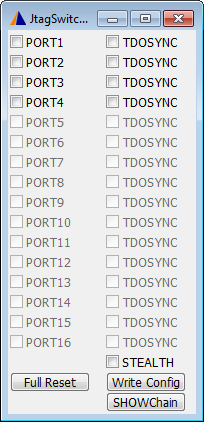
\includegraphics[scale=0.35]{../png/jswitch_dialog_deselect.png}};
\node [anchor=north west] at (dialog1.north east) (showchain1) {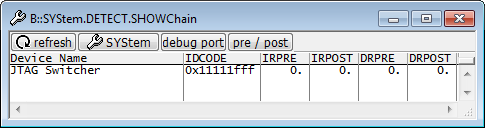
\includegraphics[scale=0.33]{../png/jswitch_showchain_deselect.png}};
\node [anchor=west] at ([xshift=0.5em]showchain1.east) (text1) {No PORT/TAP selected};
\node [anchor=north west] at ([xshift=1em,yshift=-1em]showchain1.south west) (dialog2) {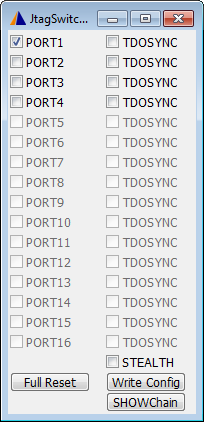
\includegraphics[scale=0.35]{../png/jswitch_dialog_port1.png}};
\node [anchor=north west] at (dialog2.north east) (showchain2) {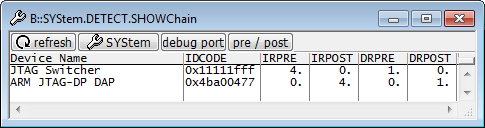
\includegraphics[scale=0.33]{../png/jswitch_showchain_port1.png}};
\node [anchor=west] at ([xshift=0.5em]showchain2.east) (text2) {First PORT/TAP selected};
\node [anchor=north west] at ([xshift=1em,yshift=-1em]showchain2.south west) (dialog3) {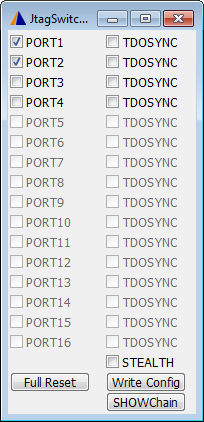
\includegraphics[scale=0.35]{../png/jswitch_dialog_port12.png}};
\node [anchor=north west] at (dialog3.north east) (showchain3) {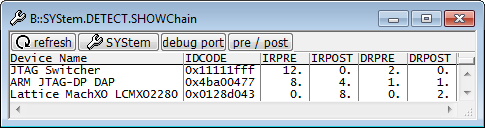
\includegraphics[scale=0.33]{../png/jswitch_showchain_port12.png}};
\node [anchor=west,align=center] at ([xshift=0.5em]showchain3.east) (text3) {PORT/TAP\\ \textbf{1 \& 2}\\ selected};
\node [anchor=north west,align=left] at ([xshift=1em,yshift=-1em]showchain3.south west) {Dialog for interactive Usage \\ part of JTAG Switcher download \\ \texttt{DO <...>/lb\_cmm/jswitch\_dialog.cmm}};
\begin{scope}[on background layer]
\fill [rounded corners,ltb_blue!20] ([yshift=0.2em]dialog1.north) -| ([xshift=0.2em]text1.east) |- ([yshift=-0.2em]showchain1.south) -| ([xshift=0.2em]dialog1.east) |- ([yshift=-0.2em]dialog1.south) -| ([xshift=-0.2em]dialog1.west) |- ([yshift=0.2em]dialog1.north);
\fill [rounded corners,ltb_blue!20] ([yshift=0.2em]dialog2.north) -| ([xshift=0.2em]text2.east) |- ([yshift=-0.2em]showchain2.south) -| ([xshift=0.2em]dialog2.east) |- ([yshift=-0.2em]dialog2.south) -| ([xshift=-0.2em]dialog2.west) |- ([yshift=0.2em]dialog2.north);
\fill [rounded corners,ltb_blue!20] ([yshift=0.2em]dialog3.north) -| ([xshift=0.2em]text3.east) |- ([yshift=-0.2em]showchain3.south) -| ([xshift=0.2em]dialog3.east) |- ([yshift=-0.2em]dialog3.south) -| ([xshift=-0.2em]dialog3.west) |- ([yshift=0.2em]dialog3.north);
\end{scope}
\end{tikzpicture}
\end{frame}

\begin{frame}[fragile]{Usage}
\begin{Verbatim}[fontsize=\tiny,commandchars=\\\{\}]
IF !(JTAG.SEQuence.EXIST(TLRJSwitchReset)&&JTAG.SEQuence.EXIST(TLRJSwitchWriteReg))
(
  DO <...>/lb_cmm/jswitch_jtagsequence_lib.cmm
)
; optional
; JTAG.SEQuence.Execute TLRJSwitchReset

JTAG.SEQuence.Execute TLRJSwitchDisableAll
JTAG.SEQuence.Execute TLRJSwitchWriteAllBanks 0x\mytikzrefnode{n1}1 <Bank1\mytikzrefnode{n2} Value> <Bank2\mytikzrefnode{n3} Value>
\end{Verbatim}
\begin{tikzpicture}[overlay]
\draw [ltb_blue,shorten <=0.3em] (n3) |- +(2em,1.0em) node [right] (t3) {PORT/TAP 9-16};
\draw [ltb_blue,shorten <=0.3em] (n2) |- ([yshift=1.2em]t3.west) node [right] (t2) {PORT/TAP 1-8};
\draw [ltb_blue,shorten <=0.3em] (n1) |- ([yshift=1.2em]t2.west) node [right] (t1) {Register SELECT};
\end{tikzpicture}
JTAG Switcher Register Bit mapping
\begin{footnotesize}
\begin{tabular}{l|c|c|c|c|c|c|c|c|c|c|c|c|c|c|c|c}
Slave TAP & \multicolumn{2}{c|}{16} & \multicolumn{2}{c|}{15} & \multicolumn{2}{c|}{14} & \multicolumn{2}{c|}{13} & \multicolumn{2}{c|}{12} & \multicolumn{2}{c|}{11} & \multicolumn{2}{c|}{10} & \multicolumn{2}{c}{9}\\
Slave TAP & \multicolumn{2}{c|}{8} & \multicolumn{2}{c|}{7} & \multicolumn{2}{c|}{6} & \multicolumn{2}{c|}{5} & \multicolumn{2}{c|}{4} & \multicolumn{2}{c|}{3} & \multicolumn{2}{c|}{2} & \multicolumn{2}{c}{1}\\
\hline
Bits & 15 & 14 & 13 & 12 & 11 & 10 & 9 & 8 & 7 & 6 & 5 & 4 & 3 & 2 & 1 & 0\\
\hline \hline
\multicolumn{15}{r|}{No Operation} & 0 & 0\\
\multicolumn{15}{r|}{Set Bit} & 0 & 1\\
\multicolumn{15}{r|}{Clear Bit} & 1 & 0\\
\multicolumn{15}{r|}{Clear Bit} & 1 & 1
\end{tabular}
\end{footnotesize}
\end{frame}

\begin{frame}{Examples}
\begin{itemize}
\item Example: Enable PORT1\\
\texttt{\footnotesize{}JTAG.SEQuence.Execute TLRJSwitchDisableAll}\\
\texttt{\footnotesize{}JTAG.SEQuence.Execute TLRJSwitchWriteAllBanks 0x1 0x1 0x0}\\
or (including disable all other ports pattern)\\
\texttt{\footnotesize{}JTAG.SEQuence.Execute TLRJSwitchWriteAllBanks 0x1 0x1|0xAAA8 0xAAAA}\\
\end{itemize}
\begin{block}{TLRJSwitchDisableAll}
The JTAG Sequences \texttt{TLRJSwitchDisableAll} \& \texttt{TLRJSwitchReset} are robust against 128 (remaining) IR-Bits in the chain (\textasciitilde{}32 ARM-SoCs).
\end{block}
\begin{block}{TLRJSwitchWriteAllBanks}
All JTAG Sequences \texttt{TLRJSwitchWrite...} must not be called when a debug session is active. The chain must include \emph{ONLY} JTAG Switcher.
\end{block}
\end{frame}

\begin{frame}{Examples}
\begin{itemize}
\item Example: Enable PORTs 4,5,9\\
\texttt{\footnotesize{}JTAG.SEQuence.Execute TLRJSwitchDisableAll}\\
\texttt{\footnotesize{}JTAG.SEQuence.Execute TLRJSwitchWriteAllBanks 0x1 0x140 0x1}
\item Example: Reset JTAG Switcher including all miscellaneous registers
\texttt{\footnotesize{}JTAG.SEQuence.Execute TLRJSwitchReset}
\item Example: Enable PORTs 4,5,9 - enable TDOSYNC for Port 4,5\\
\texttt{\footnotesize{}JTAG.SEQuence.Execute TLRJSwitchDisableAll}\\
\texttt{\footnotesize{}JTAG.SEQuence.Execute TLRJSwitchWriteAllBanks 0x2 0x140 0x2}\\
\texttt{\footnotesize{}JTAG.SEQuence.Execute TLRJSwitchWriteAllBanks 0x1 0x140 0x1}
\end{itemize}
\begin{block}{Reminder}
\texttt{TLRJSwitchDisableAll} does only reset the SELECT(=\texttt{0x1}) register, others e.g. TDO-SYNC(=\texttt{0x2}) are not affected.
\end{block}
\end{frame}

\begin{frame}[fragile]{Usage}
\begin{columns}[c]
\begin{column}{0.45\textwidth}
Debug Session configuration
\begin{Verbatim}[fontsize=\tiny,commandchars=\\\{\}]
  SYStem.CPU <SoC-Cluster>
  SYStem.CONFIG IRPRE  <>
  SYStem.CONFIG DRPRE  <>
  SYStem.CONFIG IRPOST <>
  SYStem.CONFIG DRPOST <>
  SYStem.Mode <Attach|Up>
\end{Verbatim}
ARM Coresight based System
\begin{Verbatim}[fontsize=\tiny,commandchars=\\\{\}]
  SYStem.CPU <SoC-Cluster>
  SYStem.CONFIG DAPIRPRE  <>
  SYStem.CONFIG DAPDRPRE  <>
  SYStem.CONFIG DAPIRPOST <>
  SYStem.CONFIG DAPDRPOST <>
  SYStem.Mode <Attach|Up>
\end{Verbatim}
\end{column}
\begin{column}{0.45\textwidth}
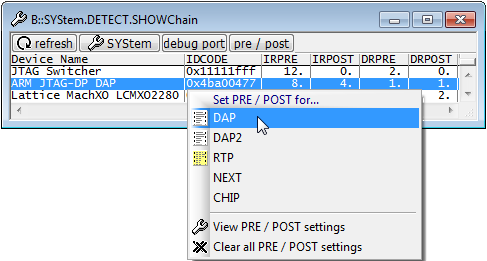
\includegraphics[width=\textwidth]{../png/jswitch_showchain_port12_prepost.png}
\end{column}
\end{columns}
\end{frame}

\subsection{Dynamic Chaining}

\begin{frame}{Dynamic Chaining}
Usecase 2: Dynamically control the Daisy-Chain from the probe
\begin{itemize}
\item Idea: Activate only one PORT/TAP at a time
\item $\Rightarrow$ Chain consists only of JTAG Switcher and current TAP of \emph{interest}
\item $\Rightarrow$ Errors from other TAPs do not propagate
\item Thus we may use JTAG Switcher as one logical multiplexer
\end{itemize}
\begin{center}
\newcommand{\jtag}[2]
{
\node [jnode,anchor=west] (jtag#1) at #2 {};
\node [right] at ([yshift=0.5em]jtag#1.west) (_jtag#1_tdi) {TDI};
\node [left] at ([yshift=0.5em]jtag#1.east) (_jtag#1_tdo) {TDO};
\node [above] at ([xshift=-1.5em]jtag#1.south) (_jtag#1_tck)  {TCK};
\node [above] at ([xshift=1.5em]jtag#1.south) (_jtag#1_tms) {TMS};
\coordinate (jtag#1_tdi) at (_jtag#1_tdi.west);
\coordinate (jtag#1_tdo) at (_jtag#1_tdo.east);
\coordinate (jtag#1_tck) at (_jtag#1_tck.south);
\coordinate (jtag#1_tms) at (_jtag#1_tms.south);
}
\tikzstyle{jnode}=[draw,rounded corners,minimum height=3.5em,minimum width=8em]
\tikzstyle{buffer}=[draw=black,fill=white,regular polygon,regular polygon sides=3,rotate=30,inner sep=0,minimum height=1.5em]

\tikzstyle{demux} = [trapezium,draw,shape border rotate=90,trapezium stretches body]
\tikzstyle{mux} = [trapezium,draw,shape border rotate=270,trapezium stretches body]
\tikzstyle{demux}+=[minimum width=6em]
\tikzstyle{mux}+=[minimum width=6em]
\begin{tikzpicture}{}
\node [draw] (control) {Controller};
\node [demux,anchor=west] at ([xshift=1em]control.east) (demux1) {};
\coordinate (demux1_out1) at ($(demux1.bottom left corner)!0.9!(demux1.bottom right corner)$);
\coordinate (demux1_out2) at ($(demux1.bottom left corner)!0.63!(demux1.bottom right corner)$);
\coordinate (demux1_out3) at ($(demux1.bottom left corner)!0.37!(demux1.bottom right corner)$);
\coordinate (demux1_out4) at ($(demux1.bottom left corner)!0.1!(demux1.bottom right corner)$);
\node [coordinate] at ($(demux1.west)$) (demux1_in) {};
\node [mux] at ($(demux1)+(5em,0)$) (mux1) {};
\coordinate (mux1_in1) at ($(mux1.bottom right corner)!0.9!(mux1.bottom left corner)$);
\coordinate (mux1_in2) at ($(mux1.bottom right corner)!0.633!(mux1.bottom left corner)$);
\coordinate (mux1_in3) at ($(mux1.bottom right corner)!0.367!(mux1.bottom left corner)$);
\coordinate (mux1_in4) at ($(mux1.bottom right corner)!0.1!(mux1.bottom left corner)$);
\coordinate (mux1_out) at ($(mux1.east)$);
\node [draw,] at ($(demux1_out1)!0.5!(mux1_in1)$) (tap1) {TAP};
\node [draw,] at ($(demux1_out2)!0.5!(mux1_in2)$) (tap2) {TAP};
\node [draw,] at ($(demux1_out3)!0.5!(mux1_in3)$) (tap3) {TAP};


\draw [<-] (control.west) -- + (-1em,0) node [left] (tdi) {\footnotesize{} TDI};
\draw [->] (control) -- (demux1_in);

\draw [->] (demux1_out1) -- (tap1);
\draw [->] (tap1) -- (mux1_in1);
\draw [->] (demux1_out2) -- (tap2);
\draw [->] (tap2) -- (mux1_in2);
\draw [->] (demux1_out3) -- (tap3);
\draw [->] (tap3) -- (mux1_in3);
\draw [->] (demux1_out4) -- (mux1_in4);

\draw [->] (mux1_out) -- +(1em,0) node [right,align=left] {\footnotesize{}TDO};
\draw [double distance=0.1em] (demux1.south) -- ($(demux1.south) + (0,-0.5em)$) node [below] (tmp1) {\footnotesize{}} -| (control.south);
\draw [double distance=0.1em] (mux1.south) |- (tmp1.north);
% \draw [densely dotted] ([xshift=0.1em]control.south) |- ([yshift=-0.2em]tmp1.north) -- +(1em,0);
% \draw [densely dotted] ([xshift=-0.1em]control.south) |- ([yshift=-0.4em]tmp1.north) -- ++(0.5em,0);
% \draw [->] ([xshift=-0.3em]control.south) |- ([yshift=-0.6em]tmp1.north) -| coordinate (tmp1) (demux3.south);
% \draw [->] (tmp1) -| (mux3.south);
\end{tikzpicture}
\end{center}
\end{frame}

\begin{frame}{Dynamic Chaining}
\begin{center}
\newcommand{\jtag}[2]
{
\node [jnode,anchor=west] (jtag#1) at #2 {};
\node [right] at ([yshift=0.5em]jtag#1.west) (_jtag#1_tdi) {TDI};
\node [left] at ([yshift=0.5em]jtag#1.east) (_jtag#1_tdo) {TDO};
\node [above] at ([xshift=-1.5em]jtag#1.south) (_jtag#1_tck)  {TCK};
\node [above] at ([xshift=1.5em]jtag#1.south) (_jtag#1_tms) {TMS};
\coordinate (jtag#1_tdi) at (_jtag#1_tdi.west);
\coordinate (jtag#1_tdo) at (_jtag#1_tdo.east);
\coordinate (jtag#1_tck) at (_jtag#1_tck.south);
\coordinate (jtag#1_tms) at (_jtag#1_tms.south);
}
\tikzstyle{jnode}=[draw,rounded corners,minimum height=3.5em,minimum width=8em]
\tikzstyle{buffer}=[draw=black,fill=white,regular polygon,regular polygon sides=3,rotate=30,inner sep=0,minimum height=1.5em]

\tikzstyle{demux} = [trapezium,draw,shape border rotate=90,trapezium stretches body]
\tikzstyle{mux} = [trapezium,draw,shape border rotate=270,trapezium stretches body]
\tikzstyle{demux}+=[minimum width=3em]
\tikzstyle{mux}+=[minimum width=3em]
\begin{tikzpicture}{}
\node [draw] (control) {Controller};
\node [demux,anchor=west] at ([xshift=1em]control.east) (demux1) {};
\node [coordinate] at ($(demux1.north east)!0.5!(demux1.bottom right corner)$) (demux1_out1) {};
\node [coordinate] at ($(demux1.south east)!0.5!(demux1.bottom left corner)$) (demux1_out2) {};
\node [coordinate] at ($(demux1.west)$) (demux1_in) {};
\node [mux] at ($(demux1)+(5em,0)$) (mux1) {};
\node [coordinate] at ($(mux1.north west)!0.5!(mux1.bottom left corner)$) (mux1_in1) {};
\node [coordinate] at ($(mux1.south west)!0.5!(mux1.bottom right corner)$) (mux1_in2) {};
\node [coordinate] at ($(mux1.east)$) (mux1_out) {};
\node [draw,] at ($(demux1_out1)!0.5!(mux1_in1)$) (tap1) {TAP};


\node [demux,densely dotted,anchor=west] at ([xshift=1em]mux1_out) (demux2) {};
\node [coordinate] at ($(demux2.north east)!0.5!(demux2.bottom right corner)$) (demux2_out1) {};
\node [coordinate] at ($(demux2.south east)!0.5!(demux2.bottom left corner)$) (demux2_out2) {};
\node [coordinate] at ($(demux2.west)$) (demux2_in) {};
\node [mux,densely dotted,anchor=west] at ([xshift=1em]demux2.east) (mux2) {};
\node [coordinate] at ($(mux2.north west)!0.5!(mux2.bottom left corner)$) (mux2_in1) {};
\node [coordinate] at ($(mux2.south west)!0.5!(mux2.bottom right corner)$) (mux2_in2) {};
\node [coordinate] at ($(mux2.east)$) (mux2_out) {};

\node [demux,anchor=west] at ([xshift=1em]mux2_out) (demux3) {};
\node [coordinate] at ($(demux3.north east)!0.5!(demux3.bottom right corner)$) (demux3_out1) {};
\node [coordinate] at ($(demux3.south east)!0.5!(demux3.bottom left corner)$) (demux3_out2) {};
\node [coordinate] at ($(demux3.west)$) (demux3_in) {};
\node [mux] at ($(demux3)+(5em,0)$) (mux3) {};
\node [coordinate] at ($(mux3.north west)!0.5!(mux3.bottom left corner)$) (mux3_in1) {};
\node [coordinate] at ($(mux3.south west)!0.5!(mux3.bottom right corner)$) (mux3_in2) {};
\node [coordinate] at ($(mux3.east)$) (mux3_out) {};
\node [draw,] at ($(demux3_out1)!0.5!(mux3_in1)$) (tap3) {TAP};

\draw [<-] (control.west) -- + (-1em,0) node [left] {\footnotesize{} TDI};
\draw [->] (control) -- (demux1_in);

\draw [->] ($(demux1_out2)$) -- ($(mux1_in2)$);
\draw [->] (demux1_out1) -- (tap1);
\draw [->] (tap1) -- (mux1_in1);

\draw [->,dotted] (mux1_out) -- (demux2_in);

\draw [->,dotted] (demux2_out2) -- (mux2_in2);

\draw [->,dotted] (mux2_out) -- (demux3_in);

\draw [->] (demux3_out1) -- (tap3);
\draw [->] (tap3) -- (mux3_in1);
\draw [->] (demux3_out2) -- (mux3_in2);

\draw [->] (mux3_out) -- +(1em,0) node [right,align=left] {\footnotesize{}TDO};
\draw [<-] (demux1.south) -- ($(demux1.south) + (0,-0.5em)$) node [below] (tmp1) {\footnotesize{}} -| ([xshift=0.3em]control.south);
\draw [<-] (mux1.south) |- (tmp1.north);
\draw [densely dotted] ([xshift=0.1em]control.south) |- ([yshift=-0.2em]tmp1.north) -- +(1em,0);
\draw [densely dotted] ([xshift=-0.1em]control.south) |- ([yshift=-0.4em]tmp1.north) -- ++(0.5em,0);
\draw [->] ([xshift=-0.3em]control.south) |- ([yshift=-0.6em]tmp1.north) -| coordinate (tmp1) (demux3.south);
\draw [->] (tmp1) -| (mux3.south);
\end{tikzpicture}
\end{center}
\begin{tikzpicture}[overlay]
\node [draw,thick,ltb_blue,inner sep=0,fit=(tap1)] (tap1_upper) {};
\node [draw,thick,ltb_orange,inner sep=0,fit=(tap3)] (tap3_upper) {};

\draw [thick,ltb_green,->] (demux1_out2) -- (mux1_in2);
\draw [thick,ltb_green,->] (demux2_out2) -- (mux2_in2);
\draw [thick,ltb_green,->] (demux3_out2) -- (mux3_in2);
\end{tikzpicture}
\begin{center}
\newcommand{\jtag}[2]
{
\node [jnode,anchor=west] (jtag#1) at #2 {};
\node [right] at ([yshift=0.5em]jtag#1.west) (_jtag#1_tdi) {TDI};
\node [left] at ([yshift=0.5em]jtag#1.east) (_jtag#1_tdo) {TDO};
\node [above] at ([xshift=-1.5em]jtag#1.south) (_jtag#1_tck)  {TCK};
\node [above] at ([xshift=1.5em]jtag#1.south) (_jtag#1_tms) {TMS};
\coordinate (jtag#1_tdi) at (_jtag#1_tdi.west);
\coordinate (jtag#1_tdo) at (_jtag#1_tdo.east);
\coordinate (jtag#1_tck) at (_jtag#1_tck.south);
\coordinate (jtag#1_tms) at (_jtag#1_tms.south);
}
\tikzstyle{jnode}=[draw,rounded corners,minimum height=3.5em,minimum width=8em]
\tikzstyle{buffer}=[draw=black,fill=white,regular polygon,regular polygon sides=3,rotate=30,inner sep=0,minimum height=1.5em]

\tikzstyle{demux} = [trapezium,draw,shape border rotate=90,trapezium stretches body]
\tikzstyle{mux} = [trapezium,draw,shape border rotate=270,trapezium stretches body]
\tikzstyle{demux}+=[minimum width=6em]
\tikzstyle{mux}+=[minimum width=6em]
\begin{tikzpicture}{}
\node [draw] (control) {Controller};
\node [demux,anchor=west] at ([xshift=1em]control.east) (demux1) {};
\coordinate (demux1_out1) at ($(demux1.bottom left corner)!0.9!(demux1.bottom right corner)$);
\coordinate (demux1_out2) at ($(demux1.bottom left corner)!0.63!(demux1.bottom right corner)$);
\coordinate (demux1_out3) at ($(demux1.bottom left corner)!0.37!(demux1.bottom right corner)$);
\coordinate (demux1_out4) at ($(demux1.bottom left corner)!0.1!(demux1.bottom right corner)$);
\node [coordinate] at ($(demux1.west)$) (demux1_in) {};
\node [mux] at ($(demux1)+(5em,0)$) (mux1) {};
\coordinate (mux1_in1) at ($(mux1.bottom right corner)!0.9!(mux1.bottom left corner)$);
\coordinate (mux1_in2) at ($(mux1.bottom right corner)!0.633!(mux1.bottom left corner)$);
\coordinate (mux1_in3) at ($(mux1.bottom right corner)!0.367!(mux1.bottom left corner)$);
\coordinate (mux1_in4) at ($(mux1.bottom right corner)!0.1!(mux1.bottom left corner)$);
\coordinate (mux1_out) at ($(mux1.east)$);
\node [draw,] at ($(demux1_out1)!0.5!(mux1_in1)$) (tap1) {TAP};
\node [draw,] at ($(demux1_out2)!0.5!(mux1_in2)$) (tap2) {TAP};
\node [draw,] at ($(demux1_out3)!0.5!(mux1_in3)$) (tap3) {TAP};


\draw [<-] (control.west) -- + (-1em,0) node [left] (tdi) {\footnotesize{} TDI};
\draw [->] (control) -- (demux1_in);

\draw [->] (demux1_out1) -- (tap1);
\draw [->] (tap1) -- (mux1_in1);
\draw [->] (demux1_out2) -- (tap2);
\draw [->] (tap2) -- (mux1_in2);
\draw [->] (demux1_out3) -- (tap3);
\draw [->] (tap3) -- (mux1_in3);
\draw [->] (demux1_out4) -- (mux1_in4);

\draw [->] (mux1_out) -- +(1em,0) node [right,align=left] {\footnotesize{}TDO};
\draw [double distance=0.1em] (demux1.south) -- ($(demux1.south) + (0,-0.5em)$) node [below] (tmp1) {\footnotesize{}} -| (control.south);
\draw [double distance=0.1em] (mux1.south) |- (tmp1.north);
% \draw [densely dotted] ([xshift=0.1em]control.south) |- ([yshift=-0.2em]tmp1.north) -- +(1em,0);
% \draw [densely dotted] ([xshift=-0.1em]control.south) |- ([yshift=-0.4em]tmp1.north) -- ++(0.5em,0);
% \draw [->] ([xshift=-0.3em]control.south) |- ([yshift=-0.6em]tmp1.north) -| coordinate (tmp1) (demux3.south);
% \draw [->] (tmp1) -| (mux3.south);
\end{tikzpicture}
\end{center}
\begin{tikzpicture}[overlay]
\node [draw,thick,ltb_blue,inner sep=0,fit=(tap1)] (tap1_lower) {};
\node [draw,thick,ltb_orange,inner sep=0,fit=(tap3)] (tap3_lower) {};
\draw [thick,ltb_blue,->] (tap1_upper.south) to[out=-90,in=100] node [fill=white,pos=0.65,inner sep=0.1em] {only TAP1 selected} (tap1_lower);
\draw [thick,ltb_orange,->] (tap3_upper.south) to[out=-90,in=20] node [fill=white,pos=0.44,inner sep=0.1em] {only TAP3 selected} (tap3_lower);
\draw [thick,ltb_green,->] (demux1_out4) -- coordinate (tmp) (mux1_in4);
\draw [shorten <=0.1em,ltb_green,<-] (tmp) to[out=-90,in=180] +(3em,-1.5em) node [right] {all PORTs/TAPs deselected};
\end{tikzpicture}
\end{frame}

\begin{frame}{Dynamic Chaining}
\begin{columns}[c]
\begin{column}{0.6\textwidth}
\begin{tikzpicture}
\node {\newcommand{\jtag}[2]
{
\node [jnode,anchor=west] (jtag#1) at #2 {};
\node [right] at ([yshift=0.5em]jtag#1.west) (_jtag#1_tdi) {TDI};
\node [left] at ([yshift=0.5em]jtag#1.east) (_jtag#1_tdo) {TDO};
\node [above] at ([xshift=-1.5em]jtag#1.south) (_jtag#1_tck)  {TCK};
\node [above] at ([xshift=1.5em]jtag#1.south) (_jtag#1_tms) {TMS};
\coordinate (jtag#1_tdi) at (_jtag#1_tdi.west);
\coordinate (jtag#1_tdo) at (_jtag#1_tdo.east);
\coordinate (jtag#1_tck) at (_jtag#1_tck.south);
\coordinate (jtag#1_tms) at (_jtag#1_tms.south);
}
\tikzstyle{jnode}=[draw,rounded corners,minimum height=3.5em,minimum width=8em]
\tikzstyle{buffer}=[draw=black,fill=white,regular polygon,regular polygon sides=3,rotate=30,inner sep=0,minimum height=1.5em]

\tikzstyle{demux} = [trapezium,draw,shape border rotate=90,trapezium stretches body]
\tikzstyle{mux} = [trapezium,draw,shape border rotate=270,trapezium stretches body]
\tikzstyle{demux}+=[minimum width=6em]
\tikzstyle{mux}+=[minimum width=6em]
\begin{tikzpicture}{}
\node [draw] (control) {Controller};
\node [demux,anchor=west] at ([xshift=1em]control.east) (demux1) {};
\coordinate (demux1_out1) at ($(demux1.bottom left corner)!0.9!(demux1.bottom right corner)$);
\coordinate (demux1_out2) at ($(demux1.bottom left corner)!0.63!(demux1.bottom right corner)$);
\coordinate (demux1_out3) at ($(demux1.bottom left corner)!0.37!(demux1.bottom right corner)$);
\coordinate (demux1_out4) at ($(demux1.bottom left corner)!0.1!(demux1.bottom right corner)$);
\node [coordinate] at ($(demux1.west)$) (demux1_in) {};
\node [mux] at ($(demux1)+(5em,0)$) (mux1) {};
\coordinate (mux1_in1) at ($(mux1.bottom right corner)!0.9!(mux1.bottom left corner)$);
\coordinate (mux1_in2) at ($(mux1.bottom right corner)!0.633!(mux1.bottom left corner)$);
\coordinate (mux1_in3) at ($(mux1.bottom right corner)!0.367!(mux1.bottom left corner)$);
\coordinate (mux1_in4) at ($(mux1.bottom right corner)!0.1!(mux1.bottom left corner)$);
\coordinate (mux1_out) at ($(mux1.east)$);
\node [draw,] at ($(demux1_out1)!0.5!(mux1_in1)$) (tap1) {TAP};
\node [draw,] at ($(demux1_out2)!0.5!(mux1_in2)$) (tap2) {TAP};
\node [draw,] at ($(demux1_out3)!0.5!(mux1_in3)$) (tap3) {TAP};


\draw [<-] (control.west) -- + (-1em,0) node [left] (tdi) {\footnotesize{} TDI};
\draw [->] (control) -- (demux1_in);

\draw [->] (demux1_out1) -- (tap1);
\draw [->] (tap1) -- (mux1_in1);
\draw [->] (demux1_out2) -- (tap2);
\draw [->] (tap2) -- (mux1_in2);
\draw [->] (demux1_out3) -- (tap3);
\draw [->] (tap3) -- (mux1_in3);
\draw [->] (demux1_out4) -- (mux1_in4);

\draw [->] (mux1_out) -- +(1em,0) node [right,align=left] {\footnotesize{}TDO};
\draw [double distance=0.1em] (demux1.south) -- ($(demux1.south) + (0,-0.5em)$) node [below] (tmp1) {\footnotesize{}} -| (control.south);
\draw [double distance=0.1em] (mux1.south) |- (tmp1.north);
% \draw [densely dotted] ([xshift=0.1em]control.south) |- ([yshift=-0.2em]tmp1.north) -- +(1em,0);
% \draw [densely dotted] ([xshift=-0.1em]control.south) |- ([yshift=-0.4em]tmp1.north) -- ++(0.5em,0);
% \draw [->] ([xshift=-0.3em]control.south) |- ([yshift=-0.6em]tmp1.north) -| coordinate (tmp1) (demux3.south);
% \draw [->] (tmp1) -| (mux3.south);
\end{tikzpicture}};

\node [anchor=south,draw,thick,ltb_blue,rounded corners,label={[ltb_blue]\footnotesize{}Session1},yshift=1.0em] at (control.north |- demux1.north) (session1) {\begin{tikzpicture}
\path (0,0) [fill,rounded corners=0.15em,black!70] -- (1em,0em) -- (1.4em,2.1em) -- (0em,0em) -- (0.5em,0em);
\path (1.5em,0) [fill,rounded corners=0.15em,black!40] -- (2.8em,0) -- (1.5em,2.1em) -- (1.15em,0em) -- +(0.5em,0);
\end{tikzpicture}
};
\node [anchor=west,draw,thick,ltb_green,rounded corners,label={[ltb_green]\footnotesize{}Session2}] at ([xshift=0.25em]session1.east) (session2) {\begin{tikzpicture}
\path (0,0) [fill,rounded corners=0.15em,black!70] -- (1em,0em) -- (1.4em,2.1em) -- (0em,0em) -- (0.5em,0em);
\path (1.5em,0) [fill,rounded corners=0.15em,black!40] -- (2.8em,0) -- (1.5em,2.1em) -- (1.15em,0em) -- +(0.5em,0);
\end{tikzpicture}
};
\node [anchor=west,draw,thick,ltb_orange,rounded corners,label={[ltb_orange]\footnotesize{}Session3}] at ([xshift=0.25em]session2.east) (session3) {\begin{tikzpicture}
\path (0,0) [fill,rounded corners=0.15em,black!70] -- (1em,0em) -- (1.4em,2.1em) -- (0em,0em) -- (0.5em,0em);
\path (1.5em,0) [fill,rounded corners=0.15em,black!40] -- (2.8em,0) -- (1.5em,2.1em) -- (1.15em,0em) -- +(0.5em,0);
\end{tikzpicture}
};
\node [draw,thick,ltb_blue,inner sep=0,fit=(tap1)] {};
\node [draw,thick,ltb_green,inner sep=0,fit=(tap2)] {};
\node [draw,thick,ltb_orange,inner sep=0,fit=(tap3)] {};
\draw [ltb_blue,->] (session1.south) to[out=-10,in=180] (tap1.west);
\draw [ltb_green,->] (session2.south) to[out=0,in=180] (tap2.west);
\draw [ltb_orange,->] (session3.south) to[out=-45,in=10] (tap3.east);
\node [draw,thick,ltb_red,inner sep=0,fit=(control)] {};
\draw [ltb_red,->] (session1.south) -- +(0,-0.4em) coordinate (intersection) -- (session1.south |- control.north);
\draw [ltb_red] (intersection) -| (session2.south);
\draw [ltb_red] (intersection) -| (session3.south);
\end{tikzpicture}
\end{column}
\begin{column}{0.4\textwidth}
\begin{itemize}
\item Every Debug session connects (ideally) to only one TAP
\item The probe (e.g. TRACE32) needs also to control the JTAG Switcher
\item $\Rightarrow$ We can dynamically start debug-sessions without prior Daisy-Chain configuration
\end{itemize}
\end{column}
\end{columns}
\end{frame}

\begin{frame}{Dynamic Chaining}
\begin{columns}[c]
\begin{column}{0.6\textwidth}
\begin{tikzpicture}
\node {\newcommand{\jtag}[2]
{
\node [jnode,anchor=west] (jtag#1) at #2 {};
\node [right] at ([yshift=0.5em]jtag#1.west) (_jtag#1_tdi) {TDI};
\node [left] at ([yshift=0.5em]jtag#1.east) (_jtag#1_tdo) {TDO};
\node [above] at ([xshift=-1.5em]jtag#1.south) (_jtag#1_tck)  {TCK};
\node [above] at ([xshift=1.5em]jtag#1.south) (_jtag#1_tms) {TMS};
\coordinate (jtag#1_tdi) at (_jtag#1_tdi.west);
\coordinate (jtag#1_tdo) at (_jtag#1_tdo.east);
\coordinate (jtag#1_tck) at (_jtag#1_tck.south);
\coordinate (jtag#1_tms) at (_jtag#1_tms.south);
}
\tikzstyle{jnode}=[draw,rounded corners,minimum height=3.5em,minimum width=8em]
\tikzstyle{buffer}=[draw=black,fill=white,regular polygon,regular polygon sides=3,rotate=30,inner sep=0,minimum height=1.5em]

\tikzstyle{demux} = [trapezium,draw,shape border rotate=90,trapezium stretches body]
\tikzstyle{mux} = [trapezium,draw,shape border rotate=270,trapezium stretches body]
\tikzstyle{demux}+=[minimum width=6em]
\tikzstyle{mux}+=[minimum width=6em]
\begin{tikzpicture}{}
\node [draw] (control) {Controller};
\node [demux,anchor=west] at ([xshift=1em]control.east) (demux1) {};
\coordinate (demux1_out1) at ($(demux1.bottom left corner)!0.9!(demux1.bottom right corner)$);
\coordinate (demux1_out2) at ($(demux1.bottom left corner)!0.63!(demux1.bottom right corner)$);
\coordinate (demux1_out3) at ($(demux1.bottom left corner)!0.37!(demux1.bottom right corner)$);
\coordinate (demux1_out4) at ($(demux1.bottom left corner)!0.1!(demux1.bottom right corner)$);
\node [coordinate] at ($(demux1.west)$) (demux1_in) {};
\node [mux] at ($(demux1)+(5em,0)$) (mux1) {};
\coordinate (mux1_in1) at ($(mux1.bottom right corner)!0.9!(mux1.bottom left corner)$);
\coordinate (mux1_in2) at ($(mux1.bottom right corner)!0.633!(mux1.bottom left corner)$);
\coordinate (mux1_in3) at ($(mux1.bottom right corner)!0.367!(mux1.bottom left corner)$);
\coordinate (mux1_in4) at ($(mux1.bottom right corner)!0.1!(mux1.bottom left corner)$);
\coordinate (mux1_out) at ($(mux1.east)$);
\node [draw,] at ($(demux1_out1)!0.5!(mux1_in1)$) (tap1) {TAP};
\node [draw,] at ($(demux1_out2)!0.5!(mux1_in2)$) (tap2) {TAP};
\node [draw,] at ($(demux1_out3)!0.5!(mux1_in3)$) (tap3) {TAP};


\draw [<-] (control.west) -- + (-1em,0) node [left] (tdi) {\footnotesize{} TDI};
\draw [->] (control) -- (demux1_in);

\draw [->] (demux1_out1) -- (tap1);
\draw [->] (tap1) -- (mux1_in1);
\draw [->] (demux1_out2) -- (tap2);
\draw [->] (tap2) -- (mux1_in2);
\draw [->] (demux1_out3) -- (tap3);
\draw [->] (tap3) -- (mux1_in3);
\draw [->] (demux1_out4) -- (mux1_in4);

\draw [->] (mux1_out) -- +(1em,0) node [right,align=left] {\footnotesize{}TDO};
\draw [double distance=0.1em] (demux1.south) -- ($(demux1.south) + (0,-0.5em)$) node [below] (tmp1) {\footnotesize{}} -| (control.south);
\draw [double distance=0.1em] (mux1.south) |- (tmp1.north);
% \draw [densely dotted] ([xshift=0.1em]control.south) |- ([yshift=-0.2em]tmp1.north) -- +(1em,0);
% \draw [densely dotted] ([xshift=-0.1em]control.south) |- ([yshift=-0.4em]tmp1.north) -- ++(0.5em,0);
% \draw [->] ([xshift=-0.3em]control.south) |- ([yshift=-0.6em]tmp1.north) -| coordinate (tmp1) (demux3.south);
% \draw [->] (tmp1) -| (mux3.south);
\end{tikzpicture}};

\node [anchor=south,draw,thick,ltb_blue,rounded corners,label={[ltb_blue]\footnotesize{}Session1},yshift=1.0em] at (control.north |- demux1.north) (session1) {\begin{tikzpicture}
\path (0,0) [fill,rounded corners=0.15em,black!70] -- (1em,0em) -- (1.4em,2.1em) -- (0em,0em) -- (0.5em,0em);
\path (1.5em,0) [fill,rounded corners=0.15em,black!40] -- (2.8em,0) -- (1.5em,2.1em) -- (1.15em,0em) -- +(0.5em,0);
\end{tikzpicture}
};
\node [anchor=west,draw,thick,ltb_green,rounded corners,label={[ltb_green]\footnotesize{}Session2}] at ([xshift=0.25em]session1.east) (session2) {\begin{tikzpicture}
\path (0,0) [fill,rounded corners=0.15em,black!70] -- (1em,0em) -- (1.4em,2.1em) -- (0em,0em) -- (0.5em,0em);
\path (1.5em,0) [fill,rounded corners=0.15em,black!40] -- (2.8em,0) -- (1.5em,2.1em) -- (1.15em,0em) -- +(0.5em,0);
\end{tikzpicture}
};
\node [anchor=west,draw,thick,ltb_orange,rounded corners,label={[ltb_orange]\footnotesize{}Session3}] at ([xshift=0.25em]session2.east) (session3) {\begin{tikzpicture}
\path (0,0) [fill,rounded corners=0.15em,black!70] -- (1em,0em) -- (1.4em,2.1em) -- (0em,0em) -- (0.5em,0em);
\path (1.5em,0) [fill,rounded corners=0.15em,black!40] -- (2.8em,0) -- (1.5em,2.1em) -- (1.15em,0em) -- +(0.5em,0);
\end{tikzpicture}
};
\node [draw,thick,ltb_blue,inner sep=0,fit=(tap1)] {};
\node [draw,thick,ltb_green,inner sep=0,fit=(tap2)] {};
\node [draw,thick,ltb_orange,inner sep=0,fit=(tap3)] {};
\draw [ltb_blue,->] (session1.south) to[out=-10,in=180] (tap1.west);
\draw [ltb_green,->] (session2.south) to[out=0,in=180] (tap2.west);
\draw [ltb_orange,->] (session3.south) to[out=-45,in=10] (tap3.east);
\node [draw,thick,ltb_red,inner sep=0,fit=(control)] {};
\draw [ltb_red,->] (session1.south) -- +(0,-0.4em) coordinate (intersection) -- (session1.south |- control.north);
\draw [ltb_red] (intersection) -| (session2.south);
\draw [ltb_red] (intersection) -| (session3.south);
\end{tikzpicture}
\begin{tikzpicture}[overlay]
\draw [draw,thick,ltb_red,shorten >=-0.2em,shorten <=-0.2em] (tap1.south west) -- (tap1.north east);
\draw [draw,thick,ltb_red,shorten >=-0.2em,shorten <=-0.2em] (tap1.south east) -- (tap1.north west);
\draw [draw,thick,ltb_red,shorten >=-0.2em,shorten <=-0.2em] (session1.south west) -- (session1.north east);
\draw [draw,thick,ltb_red,shorten >=-0.2em,shorten <=-0.2em] (session1.south east) -- (session1.north west);
\end{tikzpicture}
\end{column}
\begin{column}{0.4\textwidth}
\begin{itemize}
\item In case one TAP has an (unlikely) error while the communication is active only this session is affected
\item Example: TAP 1 in error state\\$\Rightarrow$ Session 2 \& Session 3 remain active
\end{itemize}
\end{column}
\end{columns}
\end{frame}

\begin{frame}{Dynamic Chaining}
\vspace{-2.5em}
\begin{columns}[t]
\begin{column}{0.5\textwidth}
\begin{center}\textbf{PRO}\end{center}
\begin{itemize}
\item No \emph{pre-initialization} required, configuration can be written by probe on demand
\item We can dynamically \emph{add} sessions
\item Speed limitiations (maximum TCK) of one TAP does not propagate
\item Better performance due to shorter Daisy-Chain length
\end{itemize}
\end{column}
\begin{column}{0.5\textwidth}
\begin{center}\textbf{CON}\end{center}
\begin{itemize}
\item Probe requires support for JTAG Switcher
\end{itemize}
\end{column}
\end{columns}
\end{frame}

\begin{frame}{Dynamic Chaining}
Sequence - initial Connect\\(TRACE32: \texttt{SYStem.CONFIG.MULTITAP JtagSEQuence Attach})
\begin{itemize}
\item Bring possible remaining Daisy-Chained TAPs into a safe state\\(JTAG BYPASS)
\item Disable all possibly activated JTAG Switcher PORTs\\(Reset all SELECT registers=\texttt{0x7})
\item [optional] Write JTAG Switcher miscellaneous configuration registers (e.g. TDOSYNC)
\item Write SELECT Register (Set Bit) and apply configuration
\item Test-Logic-Reset of Slave-Port-TAP
\end{itemize}
\end{frame}

\begin{frame}{Dynamic Chaining}
Sequence - activate PORT\\ (TRACE32: \texttt{SYStem.CONFIG.MULTITAP JtagSEQuence SELect})
\begin{itemize}
\item Write SELECT Register (Set Bit) and apply configuration
\item Probe operation ...
\end{itemize}
Sequence - deactivate PORT\\ (TRACE32: \texttt{SYStem.CONFIG.MULTITAP JtagSEQuence DeSELect})
\begin{itemize}
\item Probe operation ...
\item [either]Disable all activated JTAG Switcher PORTs\\(Reset all SELECT registers=\texttt{0x7})
\item [or]Write SELECT Register (Clear Bit) and apply configuration
\end{itemize}
\end{frame}

\begin{frame}[fragile]{Dynamic Chaining - TRACE32}
Usage:\\
\begin{Verbatim}[fontsize=\footnotesize,commandchars=\\\{\}]
  SYStem.CPU <SoC-Cluster>
  DO <...>/lb\_cmm/jswitch\_multitap\_jtagsequence.cmm PORT=<x>
  SYStem.Mode <Attach|Up>
\end{Verbatim}
The script \texttt{jswitch\_multitap\_jtagsequence.cmm} patches all required settings to control JTAG Switcher into the current TRACE32 session.
\begin{tikzpicture}
\node (multitap) {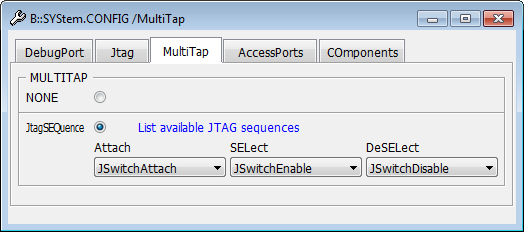
\includegraphics[width=0.5\textwidth]{../png/jswitch_sys_config_multitap.png}};
\node [anchor=north west] at (multitap.north east) (jseq) {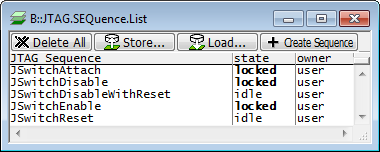
\includegraphics[width=0.35\textwidth]{../png/jswitch_multitap_sequence_list.png}};
\draw ($(multitap.north west)!0.2!(multitap.north east)$) -- + (0,0);
\draw let 
  \p1 = ($(multitap.north west)!0.19!(multitap.north east)$),
  \p2 = ($(multitap.south west)!0.41!(multitap.north west)$),
  \p3 = ($(multitap.north west)!0.435!(multitap.north east)$),
  \p4 = ($(multitap.south west)!0.25!(multitap.north west)$)
in [ltb_red]
  (\x1,\y2) -| (\x3,\y4) -| (\x1,\y2);
\draw let 
  \p1 = ($(multitap.north west)!0.44!(multitap.north east)$),
  \p2 = ($(multitap.south west)!0.41!(multitap.north west)$),
  \p3 = ($(multitap.north west)!0.6825!(multitap.north east)$),
  \p4 = ($(multitap.south west)!0.25!(multitap.north west)$)
in [ltb_red]
  (\x1,\y2) -| (\x3,\y4) -| (\x1,\y2);
\draw let 
  \p1 = ($(multitap.north west)!0.6875!(multitap.north east)$),
  \p2 = ($(multitap.south west)!0.41!(multitap.north west)$),
  \p3 = ($(multitap.north west)!0.9325!(multitap.north east)$),
  \p4 = ($(multitap.south west)!0.25!(multitap.north west)$)
in [ltb_red]
  (\x1,\y2) -| (\x3,\y4) -| (\x1,\y2);
\end{tikzpicture}
\end{frame}

\begin{frame}[fragile]{Examples}
Example: STM32F103 on Port 1\\
\begin{Verbatim}[fontsize=\tiny,commandchars=\\\{\}]
  SYStem.CPU STM32F103
  DO <...>/lb\_cmm/jswitch\_multitap\_jtagsequence.cmm PORT=1
  SYStem.Mode <Attach|Up>
\end{Verbatim}

Example: STM32F103 on Port 1, activate TDOSYNC\\
\begin{Verbatim}[fontsize=\tiny,commandchars=\\\{\}]
  SYStem.CPU STM32F103
  DO <...>/lb\_cmm/jswitch\_multitap\_jtagsequence.cmm PORT=1 TDOSYNC
  SYStem.Mode <Attach|Up>
\end{Verbatim}

Example: Daisy-Chain on Port 1\\JTAG Switcher -> FPGA (IR=5, DR=1) -> STM32F103 -> JTAG Switcher\\
\begin{Verbatim}[fontsize=\tiny,commandchars=\\\{\}]
  SYStem.CPU STM32F103
  DO <...>/lb\_cmm/jswitch\_multitap\_jtagsequence.cmm PORT=1 IRPOST=5 DRPOST=1
  SYStem.Mode <Attach|Up>
\end{Verbatim}
\end{frame}

\begin{frame}[fragile]{Examples}
Example: Daisy-Chain on Port 5\\JTAG Switcher -> STM32F103 -> FPGA (IR=5, DR=1) -> JTAG Switcher\\
\begin{Verbatim}[fontsize=\tiny,commandchars=\\\{\}]
  SYStem.CPU STM32F103
  DO <...>/lb\_cmm/jswitch\_multitap\_jtagsequence.cmm PORT=5 IRPRE=5 DRPRE=1
  SYStem.Mode <Attach|Up>
\end{Verbatim}
Example: ZYNQ-Ultrascale+ on Port 4\\JTAG Switcher -> SoC internal Daisy-Chain -> JTAG Switcher\\
\begin{Verbatim}[fontsize=\tiny,commandchars=\\\{\}]
  SYStem.CPU ZYNQ-ULTRASCALE+-APU
  DO <...>/lb\_cmm/jswitch\_multitap\_jtagsequence.cmm PORT=4 IRPOST=12 DRPOST=1
  SYStem.Mode <Attach|Up>
\end{Verbatim}
\end{frame}


\section{Advanced Features}
\begin{frame}
\frametitle{Overview}
\tableofcontents[hideallsubsections,currentsection]
\end{frame}
\subsection{TDOSYNC}
\begin{frame}{TDOSYNC}
\begin{itemize}
\item Simplified timing model of a JTAG Switcher Daisy-Chain with two Slave TAPs/PORTs activated
\item Two worst case timings $t_{delay,dut,dut}$ and $t_{delay,dut,probe}$\\Includes: level shifters, signal lines and delay in Slave TAP  \& FPGA
\item<2->[$\Rightarrow$] TDOSYNC - adds a synchronization register (virtual IR/DR Bit)
\end{itemize}
\begin{center}
%{\fontsize{6pt}{5}\selectfont \tikzset{font={\fontsize{6pt}{5}\selectfont}}
\resizebox{\textwidth}{!}{
\newcommand{\jtagsyncnode}[4]{
\node [anchor=base west,draw,align=center,minimum height=3em,minimum width=2em,#4] (#2) at (#1) {#3};
\coordinate (#2_tck) at ($(#2.north west)!0.75!(#2.south west)$);
\coordinate (#2_tdi) at ($(#2.north west)!0.25!(#2.south west)$);
\path (#2_tdi) -| coordinate (#2_tdo) (#2.east);
\draw (#2_tck) -- +(0,0.5em) -- +(0.7em,0) -- +(0,-0.5em) -- (#2_tck);
}
\newcommand{\jtagsync}[2]{\jtagsyncnode{#1}{reg#2}{S\\D}{text=white}}
\newcommand{\jtagsimple}[3]{
\node [anchor=base west,draw,align=center,minimum height=3em,minimum width=2em] at (#1) (#2) {#3};
\coordinate (#2_tdi) at ($(#2.north west)!0.25!(#2.south west)$);
\path (#2_tdi) -| coordinate (#2_tdo) (#2.east);
}
\newcommand{\tdosyncmodel}[2]
{
\jtagsyncnode{#1}{probe_in}{PROBE\\TDI}{}
\jtagsyncnode{[xshift=2em]probe_in.base east}{fpga1}{JTAG\\Switcher}{inner xsep=1.0em}
\jtagsyncnode{[xshift=2em]fpga1.base east}{dut1}{DUT\\TAP}{inner xsep=1.0em}
\ifthenelse{#2}
{
  \jtagsync{[xshift=2em]dut1.base east}{2}
  \jtagsimple{[xshift=1em]reg2.base east}{fpga2}{JTAG\\Switcher};
}
{
  \jtagsimple{[xshift=5em]dut1.base east}{fpga2}{JTAG\\Switcher};
}
\jtagsyncnode{[xshift=2em]fpga2.base east}{dut2}{DUT\\TAP}{inner xsep=1.0em};
\ifthenelse{#2}
{
  \jtagsync{[xshift=2em]dut2.base east}{3}
  \jtagsimple{[xshift=1em]reg3.base east}{fpga3}{JTAG\\Switcher};
}
{
  \jtagsimple{[xshift=5em]dut2.base east}{fpga3}{JTAG\\Switcher};
}
\jtagsyncnode{[xshift=2em]fpga3.base east}{probe_out}{PROBE\\TDO}{};
\draw [thick,->] (probe_in_tdo) -- node [above] {\footnotesize{}TDI} (fpga1_tdi);
\draw [thick,->] (fpga1_tdo) -- (dut1_tdi);
\ifthenelse{#2}{
  \draw [thick,->] (dut1_tdo) -- (reg2_tdi);
  \draw [thick,->] (reg2_tdo) -- (fpga2_tdi);
}{
  \draw [thick,->] (dut1_tdo) -- (fpga2_tdi);
}
\draw [thick,->] (fpga2_tdo) -- (dut2_tdi);
\ifthenelse{#2}{
  \draw [thick,->] (dut2_tdo) -- (reg3_tdi);
  \draw [thick,->] (reg3_tdo) -- (fpga3_tdi);
}{
  \draw [thick,->] (dut2_tdo) -- (fpga3_tdi);
}
\draw [thick,->] (fpga3_tdo) -- node [above] {\footnotesize{}TDO} (probe_out_tdi);
\draw [thick] (probe_in_tck) -| ++(-0.5em,-2em) coordinate (tck_inters)-- + (-1em,0) node [left] {TCK};
\draw [thick] (fpga1_tck) -- ++(-0.5em,0) |- (tck_inters);
\draw [thick] (dut1_tck) -- ++(-0.5em,0) |- (tck_inters);
\ifthenelse{#2}{
  \draw [thick] (reg2_tck) -- ++(-0.5em,0) |- (tck_inters);
}{}
\draw [thick] (dut2_tck) -- ++(-0.5em,0) |- (tck_inters);
\ifthenelse{#2}{
  \draw [thick] (reg3_tck) -- ++(-0.5em,0) |- (tck_inters);
}{}
\draw [thick] (probe_out_tck) -- ++(-0.5em,0) |- (tck_inters);
}

\begin{tikzpicture}[]
\tdosyncmodel{0,0}{1=0}
\draw [shorten >=-0.3em] (dut1.north east) -- +(0,2em) coordinate (t1);
\draw [shorten >=-0.3em] (dut2.north west) -- +(0,2em) coordinate (t2);
\draw [<->] (t1) -- node [above,] {\footnotesize{}$t_{delay,dut,dut}$} (t2);

\draw [shorten >=-0.3em] (dut2.north east) -- +(0,2em) coordinate (t1);
\draw [shorten >=-0.3em] (probe_out.north west) -- +(0,2em) coordinate (t2);
\draw [<->] (t1) -- node [above,] {\footnotesize{}$t_{delay,dut,probe}$} (t2);

\onslide<2->{
\tdosyncmodel{0,-6em}{1=1}

\node [fit=(reg2)(fpga2),draw,rounded corners,ltb_blue,thick] {};
\node [fit=(reg3)(fpga3),draw,rounded corners,ltb_blue,thick] {};
}


\end{tikzpicture}
}
\end{center}
\end{frame}

\begin{frame}{TDOSYNC Static Chaining}
\begin{itemize}
\item TDOSYNC is available in the JTAG Switcher Dialog
\item TDOSYNC can also be activated using the \texttt{jswitch\_jtag\_sequence\_lib.cmm} \& \texttt{JTAG.SEQuence.Execute}\\ compare examples in Static Chaining section
\item The inserted TDOSYNC register needs to be configured in the\\ \texttt{SYStem.CONFIG [DAP]IRPRE}\\ \texttt{SYStem.CONFIG [DAP]DRPRE}
\end{itemize}
\end{frame}

\begin{frame}{TDOSYNC Static Chaining}
\begin{itemize}
\item TDOSYNC is available in the JTAG Switcher Dialog
\item TDOSYNC can also be activated using the \texttt{jswitch\_jtag\_sequence\_lib.cmm} \& \texttt{JTAG.SEQuence.Execute}\\ compare examples in Static Chaining section
\item The inserted TDOSYNC register needs to be configured in the\\ \texttt{SYStem.CONFIG [DAP]IRPRE}\\ \texttt{SYStem.CONFIG [DAP]DRPRE}
\end{itemize}
\end{frame}

\begin{frame}[fragile]{TDOSYNC Static Chaining}
Example: enable PORT 1 with STM32F103, activate TDOSYNC

\begin{Verbatim}[fontsize=\tiny,commandchars=\\\{\}]
IF !(JTAG.SEQuence.EXIST(TLRJSwitchReset)&&JTAG.SEQuence.EXIST(TLRJSwitchWriteReg))
(
  DO <...>/lb_cmm/jswitch_jtagsequence_lib.cmm
)
\textcolor{olive}{; optional}
; JTAG.SEQuence.Execute TLRJSwitchReset

JTAG.SEQuence.Execute TLRJSwitchDisableAll
JTAG.SEQuence.Execute TLRJSwitchWriteAllBanks 0x2 0x1 \textcolor{olive}{; TDOSYNC}
JTAG.SEQuence.Execute TLRJSwitchWriteAllBanks 0x1 0x1 \textcolor{olive}{; SELECT}

SYStem.CPU STM32F103
SYStem.CONFIG DAPIRPOST 4. \textcolor{olive}{; JTAG Switcher}
SYStem.CONFIG DAPDRPOST 1. \textcolor{olive}{; JTAG Switcher}
SYStem.CONFIG DAPIRPRE 1.  \textcolor{olive}{; TDOSYNC}
SYStem.CONFIG DAPDRPRE 1.  \textcolor{olive}{; TDOSYNC}
SYStem.Mode <Attach|Up>
\end{Verbatim}
\end{frame}

\begin{frame}[fragile]{TDOSYNC Dynamic Chaining}
\begin{itemize}
\item TDOSYNC is available as a parameter in \texttt{DO <...>/lb\_cmm/jswitch\_multitap\_jtagsequence.cmm}
\item Daisy-Chaining paramters are automatically calculated
\end{itemize}
Example: enable PORT 1 with STM32F103, activate TDOSYNC
\begin{Verbatim}[fontsize=\tiny,commandchars=\\\{\}]
SYStem.CPU STM32F103
DO <...>/lb_cmm/jswitch_multitap_jtagsequence.cmm PORT=1 TDOSYNC
SYStem.Mode <Attach|Up>
\end{Verbatim}
\end{frame}

\subsection{STEALTH}
\begin{frame}{STEALTH Mode}
\begin{itemize}
\item Some SoCs require to be \emph{first} in chain
\item Examples: TriCore, C166, possibly others
\item In order to daisy-chain these devices, STEALTH mode hides JTAG Switcher in the Daisy-Chain
\item[$\Rightarrow$] First enabled PORT becomes first in chain
\end{itemize}
\begin{center}
\newcommand{\jtag}[2]
{
\node [jnode,anchor=west] (jtag#1) at #2 {};
\node [right] at ([yshift=0.5em]jtag#1.west) (_jtag#1_tdi) {TDI};
\node [left] at ([yshift=0.5em]jtag#1.east) (_jtag#1_tdo) {TDO};
\node [above] at ([xshift=-1.5em]jtag#1.south) (_jtag#1_tck)  {TCK};
\node [above] at ([xshift=1.5em]jtag#1.south) (_jtag#1_tms) {TMS};
\coordinate (jtag#1_tdi) at (_jtag#1_tdi.west);
\coordinate (jtag#1_tdo) at (_jtag#1_tdo.east);
\coordinate (jtag#1_tck) at (_jtag#1_tck.south);
\coordinate (jtag#1_tms) at (_jtag#1_tms.south);
}
\tikzstyle{jnode}=[draw,rounded corners,minimum height=3.5em,minimum width=8em]
\tikzstyle{buffer}=[draw=black,fill=white,regular polygon,regular polygon sides=3,rotate=30,inner sep=0,minimum height=1.5em]

\tikzstyle{demux} = [trapezium,draw,shape border rotate=90,trapezium stretches body]
\tikzstyle{mux} = [trapezium,draw,shape border rotate=270,trapezium stretches body]
\begin{tikzpicture}{node distance=4em}
\node [demux,minimum width=3em] (demux) {};
\node [coordinate] at ($(demux.north east)!0.5!(demux.bottom right corner)$) (demux_out1) {};
\node [coordinate] at ($(demux.south east)!0.5!(demux.bottom left corner)$) (demux_out2) {};
\node [coordinate] at ($(demux.west)$) (demux_in) {};

\node [mux,,minimum width=3em,right of=demux,node distance=9em] (mux) {};
\node [coordinate] at ($(mux.north west)!0.5!(mux.bottom left corner)$) (mux_in1) {};
\node [coordinate] at ($(mux.south west)!0.5!(mux.bottom right corner)$) (mux_in2) {};
\node [coordinate] at ($(mux.east)$) (mux_out) {};
\node [draw] at ($(demux_out1)!0.5!(mux_in1)$) (jswitch) {JTAG Switcher};

\draw ($(demux_out2)$) -- ($(mux_in2)$);
\draw (demux_out1) -- (jswitch);
\draw (jswitch) -- (mux_in1);
\draw [->] ($(demux_in) + (-1em,0)$) node [left] {\footnotesize TDI} -- (demux_in);
\draw [->] (mux_out) -- ($(mux_out) + (1em,0)$) node [right] {\footnotesize TDO to Slaves};
\draw [->] ($(demux.south) + (0,-0.5em)$) node [below] {\footnotesize STEALTH} -- (demux.south);
\draw [->] ($(mux.south) + (0,-0.5em)$) node [below] {\footnotesize STEALTH} -- (mux.south);
\end{tikzpicture}
\end{center}
\end{frame}

\begin{frame}[fragile]{STEALTH Usage}
Static-Chaining: enable PORT 1 with STM32F103, activate STEALTH
\begin{Verbatim}[fontsize=\tiny,commandchars=\\\{\}]
IF !(JTAG.SEQuence.EXIST(TLRJSwitchReset)&&JTAG.SEQuence.EXIST(TLRJSwitchWriteReg))
(
  DO <...>/lb_cmm/jswitch_jtagsequence_lib.cmm
)
\textcolor{olive}{; optional}
; JTAG.SEQuence.Execute TLRJSwitchReset

JTAG.SEQuence.Execute TLRJSwitchDisableAll
JTAG.SEQuence.Execute TLRJSwitchWriteAllBanksStealth 0x1 0x1 \textcolor{olive}{; SELECT + STEALTH}

SYStem.CPU STM32F103
SYStem.Mode <Attach|Up>
\end{Verbatim}
Dynamic-Chaining: enable PORT 1 with STM32F103, activate STEALTH
\begin{Verbatim}[fontsize=\tiny,commandchars=\\\{\}]
SYStem.CPU STM32F103
DO <...>/lb_cmm/jswitch_multitap_jtagsequence.cmm PORT=1 \color{ltb_blue}{STEALTH}
SYStem.Mode <Attach|Up>
\end{Verbatim}
\end{frame}

\section{FPGA Implementation}
\begin{frame}
\frametitle{Overview}
\tableofcontents[hideallsubsections,currentsection]
\end{frame}
\begin{frame}
\begin{itemize}
\item VHDL Source available under MIT License
\item Tested on Lattice MachXO/iCE40/ECP5, Altera MAX V/10, Xilinx CoolRunner
\item IP is configured using a single VHDL file \texttt{jswitch\_config\_pkg.vhd}
\item Source: https://www.lauterbach.com/jtag\_switcher.html
\end{itemize}
\end{frame}

\begin{frame}
Example to share JTAG probe connector between FPGA and JTAG Switcher
\begin{center}
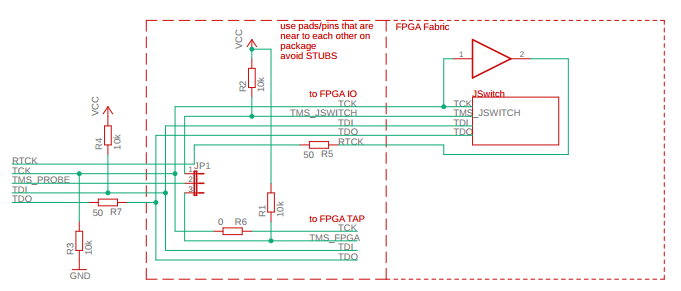
\includegraphics[width=0.8\textwidth]{../png/fpga_taps_parallel.png}
\end{center}
\end{frame}
%==============================


\end{document}
